\documentclass[11pt,a4paper]{article}

% Image mode: pdf.
% Image paths stay relative. In PDF mode, place same-basename PDF conversions
% of the chapter SVG files in the assets/ directory beside this source.

\usepackage{iftex}
\ifPDFTeX
  \PackageError{handout}{This template requires XeTeX or Tectonic}{Compile with xelatex or tectonic.}
\fi

\usepackage[a4paper,top=18mm,bottom=20mm,left=20mm,right=20mm,headsep=6mm]{geometry}
\usepackage{fontspec}
\usepackage{xeCJK}
\usepackage{amsmath}
\usepackage{unicode-math}

% Font settings are intentionally visible in the generated .tex file.
% These defaults target the macOS machine used for the released PDF.
% Change the family names when compiling on another system.
\setmainfont{Songti TC}
\setsansfont{Heiti TC}
\setmonofont{Menlo}
\setCJKmainfont{Songti TC}
\setCJKsansfont{Heiti TC}
\setCJKmonofont{Heiti TC}
\setmathfont{STIX Two Math}
\XeTeXlinebreaklocale "zh"
\XeTeXlinebreakskip=0pt plus 1pt

\usepackage{xcolor}
\definecolor{HandoutBlue}{HTML}{215A91}
\definecolor{HandoutBlueLight}{HTML}{EEF5FC}
\definecolor{HandoutGreen}{HTML}{39715A}
\definecolor{HandoutGreenLight}{HTML}{EFF8F3}
\definecolor{HandoutGold}{HTML}{8A641C}
\definecolor{HandoutGoldLight}{HTML}{FFF8E8}
\definecolor{HandoutInk}{HTML}{253142}
\definecolor{HandoutMuted}{HTML}{667085}

\usepackage{graphicx}
\makeatletter
% Pandoc 3 emits an accessibility `alt` key for raster/PDF images. Older
% graphicx releases do not know that key, so accept it without changing layout.
\@ifundefined{KV@Gin@alt}{\define@key{Gin}{alt}{}}{}
\newsavebox\pandoc@box
\newcommand*\pandocbounded[1]{%
  \sbox\pandoc@box{#1}%
  \Gscale@div\@tempa{\textheight}{\dimexpr\ht\pandoc@box+\dp\pandoc@box\relax}%
  \Gscale@div\@tempb{\linewidth}{\wd\pandoc@box}%
  \ifdim\@tempb\p@<\@tempa\p@\let\@tempa\@tempb\fi
  \ifdim\@tempa\p@<\p@\scalebox{\@tempa}{\usebox\pandoc@box}%
  \else\usebox{\pandoc@box}%
  \fi
}
\makeatother
\usepackage{float}
\floatplacement{figure}{H}
% Pandoc uses LTcaptype=none for uncaptioned longtables. The caption package
% expects that name to exist as a counter even though it is never displayed.
\newcounter{none}
\usepackage{caption}
\captionsetup[figure]{labelformat=empty,labelsep=none,font=small}

\usepackage{booktabs,longtable,array,calc}
\usepackage{etoolbox}
\makeatletter
\patchcmd\longtable{\par}{\if@noskipsec\mbox{}\fi\par}{}{}
\makeatother

\usepackage[most]{tcolorbox}
\tcbuselibrary{breakable,skins}
\newtcolorbox{HandoutLearningMap}{
  enhanced,breakable,colback=HandoutBlueLight,colframe=HandoutBlue,
  boxrule=0.8pt,arc=1.5mm,left=3mm,right=3mm,top=2mm,bottom=2mm,
  before skip=8pt,after skip=10pt
}
\newtcolorbox{HandoutWorkedExample}{
  enhanced,breakable,colback=HandoutGreenLight,colframe=HandoutGreen,
  boxrule=0.65pt,arc=1.5mm,left=3mm,right=3mm,top=2mm,bottom=2mm,
  before skip=8pt,after skip=10pt
}
\newtcolorbox{HandoutSelfCheck}{
  enhanced,breakable,colback=HandoutGoldLight,colframe=HandoutGold,
  boxrule=0.65pt,arc=1.5mm,left=3mm,right=3mm,top=2mm,bottom=2mm,
  before skip=8pt,after skip=10pt
}

\usepackage{titlesec}
\titleformat{\section}{\sffamily\bfseries\Large\color{HandoutBlue}}{}{0pt}{}
\titleformat{\subsection}{\sffamily\bfseries\large\color{HandoutInk}}{}{0pt}{}
\titleformat{\subsubsection}{\sffamily\bfseries\normalsize\color{HandoutInk}}{}{0pt}{}
\titlespacing*{\section}{0pt}{1.4em}{0.55em}
\titlespacing*{\subsection}{0pt}{1.15em}{0.45em}
\titlespacing*{\subsubsection}{0pt}{0.9em}{0.35em}
\setcounter{secnumdepth}{-\maxdimen}

\usepackage{hyperref}
\usepackage{bookmark}
\IfFileExists{xurl.sty}{\usepackage{xurl}}{}
\urlstyle{same}
\hypersetup{
  colorlinks=true,
  linkcolor=HandoutBlue,
  urlcolor=HandoutBlue,
  citecolor=HandoutBlue,
  pdftitle={數2-3 排列組合與機率},
  pdfsubject={數學},
  pdfcreator={Pandoc with the HighSchooContent LaTeX template}
}

\setlength{\parindent}{0pt}
\setlength{\parskip}{0.55em plus 0.15em minus 0.1em}
\setlength{\emergencystretch}{3em}
\setlength{\LTpre}{0.5em}
\setlength{\LTpost}{0.5em}
\renewcommand{\arraystretch}{1.18}
\providecommand{\tightlist}{%
  \setlength{\itemsep}{0pt}\setlength{\parskip}{0pt}}
\pagestyle{plain}


\begin{document}

\begin{tcolorbox}[
  enhanced,colback=white,colframe=HandoutBlue,boxrule=1.1pt,arc=2mm,
  borderline west={3pt}{0pt}{HandoutBlue},left=5mm,right=4mm,top=4mm,bottom=4mm
]
{\sffamily\small\bfseries\color{HandoutBlue}學生講義}\par
{\sffamily\bfseries\LARGE\color{HandoutInk}數2-3 排列組合與機率}\par
\vspace{0.35em}{\large 以分類、排序與樣本空間計算可能數，再用機率與期望值比較不確定結果}\par
\vspace{0.45em}{\small\color{HandoutMuted}%
科目：數學
\quad 課程：普通高中數學 第二冊
\quad 版本：學生版｜核心＋理解
\quad 校訂：2026-08-29
}\par
\vspace{0.25em}{\small\color{HandoutMuted}範圍：114 學年度數學第二冊第 3 章；邏輯與集合、計數原理、排列、重複排列、組合、二項式定理、巴斯卡三角形、樣本空間、事件、古典機率與期望值}\par
\end{tcolorbox}


\begin{HandoutLearningMap}

\subsection{本章問題與能力}\label{ux672cux7ae0ux554fux984cux8207ux80fdux529b}

\begin{enumerate}
\def\labelenumi{\arabic{enumi}.}
\tightlist
\item
  如何把敘述條件翻成邏輯關係與集合區域？
\item
  一個任務由互斥類別或連續步驟組成時，可能數如何計算？
\item
  選出的對象若有次序、職務或位置，計數公式會如何改變？
\item
  二項式展開的係數為何等於組合數？
\item
  如何建立樣本空間，讓分母與事件的分子使用同一種結果單位？
\item
  機率分布已知時，如何用期望值比較長期平均結果與公平條件？
\end{enumerate}

本章路徑：邏輯與集合 → 分類與分步計數 → 排列與組合 → 二項式係數 → 樣本空間與事件 → 古典機率 → 期望值。

\end{HandoutLearningMap}

\section{0. 本章用途：把大量可能結果整理成可計算的模型}\label{ux672cux7ae0ux7528ux9014ux628aux5927ux91cfux53efux80fdux7d50ux679cux6574ux7406ux6210ux53efux8a08ux7b97ux7684ux6a21ux578b}

密碼格式、座位安排、抽樣設計、品質檢驗與遊戲規則都有共同結構：先界定一個結果由哪些欄位或步驟構成，再辨認條件造成的分類、順序與重複。逐一列出所有結果通常很慢；計數原理把結果集合拆成互斥類別或連續步驟，直接算出總數。

實際應用會把這個總數當成搜尋空間、抽樣分母或資源配置方案數；條件改變時，計數模型也要同步更新。

機率計算需要先說清楚「一次結果」的形式。擲兩顆骰子的結果可寫成有序對 \((i,j)\)；抽出兩人若只形成小組，結果則是無序集合。樣本空間與事件使用同一種結果單位後，等可能模型中的機率才可由件數相除。

期望值把每種數值結果乘上其機率再相加。它可比較長期平均收益、設計公平計分，也能在保固成本、抽樣損耗或風險決策中把多種結果壓縮成一個平均指標。模型條件包含結果分類完整、機率總和為 \(1\)，以及每個結果的數值定義一致。

\section{1. 邏輯與集合}\label{ux908fux8f2fux8207ux96c6ux5408}

\subsection{1.1 命題、連接詞與推論}\label{ux547dux984cux9023ux63a5ux8a5eux8207ux63a8ux8ad6}

能明確判定真假的敘述稱為\textbf{命題}。命題 \(P\) 的否定記作 \(\neg P\)；「\(P\) 且 \(Q\)」記作 \(P\wedge Q\)；「\(P\) 或 \(Q\)」記作 \(P\vee Q\)，其中「或」表示至少一個成立。

條件命題 \(P\Rightarrow Q\) 表示：只要 \(P\) 成立，\(Q\) 必成立。此時 \(P\) 是 \(Q\) 的充分條件，\(Q\) 是 \(P\) 的必要條件。若 \(P\Rightarrow Q\) 與 \(Q\Rightarrow P\) 都成立，就寫成 \(P\Leftrightarrow Q\)，兩者互為充分必要條件。

否定會交換「且」與「或」：

\[
\neg(P\wedge Q)\Leftrightarrow(\neg P)\vee(\neg Q),
\]

\[
\neg(P\vee Q)\Leftrightarrow(\neg P)\wedge(\neg Q).
\]

第一式的推理是：\(P\wedge Q\) 失敗，恰好表示 \(P,Q\) 至少一個失敗。第二式同理：\(P\vee Q\) 失敗，表示兩者都失敗。這兩式稱為命題的\textbf{笛摩根律}。

\subsection{1.2 集合與運算}\label{ux96c6ux5408ux8207ux904bux7b97}

由明確對象構成的整體稱為\textbf{集合}。\(x\in A\) 表示 \(x\) 是集合 \(A\) 的元素；\(A\subseteq B\) 表示 \(A\) 的每個元素都在 \(B\) 中。有限集合 \(A\) 的元素個數記作 \(|A|\)，沒有元素的集合是空集合 \(\emptyset\)。

在全集 \(U\) 中，常用運算為

\[
A\cap B=\{x:x\in A\text{ 且 }x\in B\},
\]

\[
A\cup B=\{x:x\in A\text{ 或 }x\in B\},
\]

\[
A-B=\{x:x\in A\text{ 且 }x\notin B\},\qquad
A^c=U-A.
\]

集合與命題的結構相同：交集對應「且」，聯集對應「或」，補集對應否定。

\begin{figure}
\centering
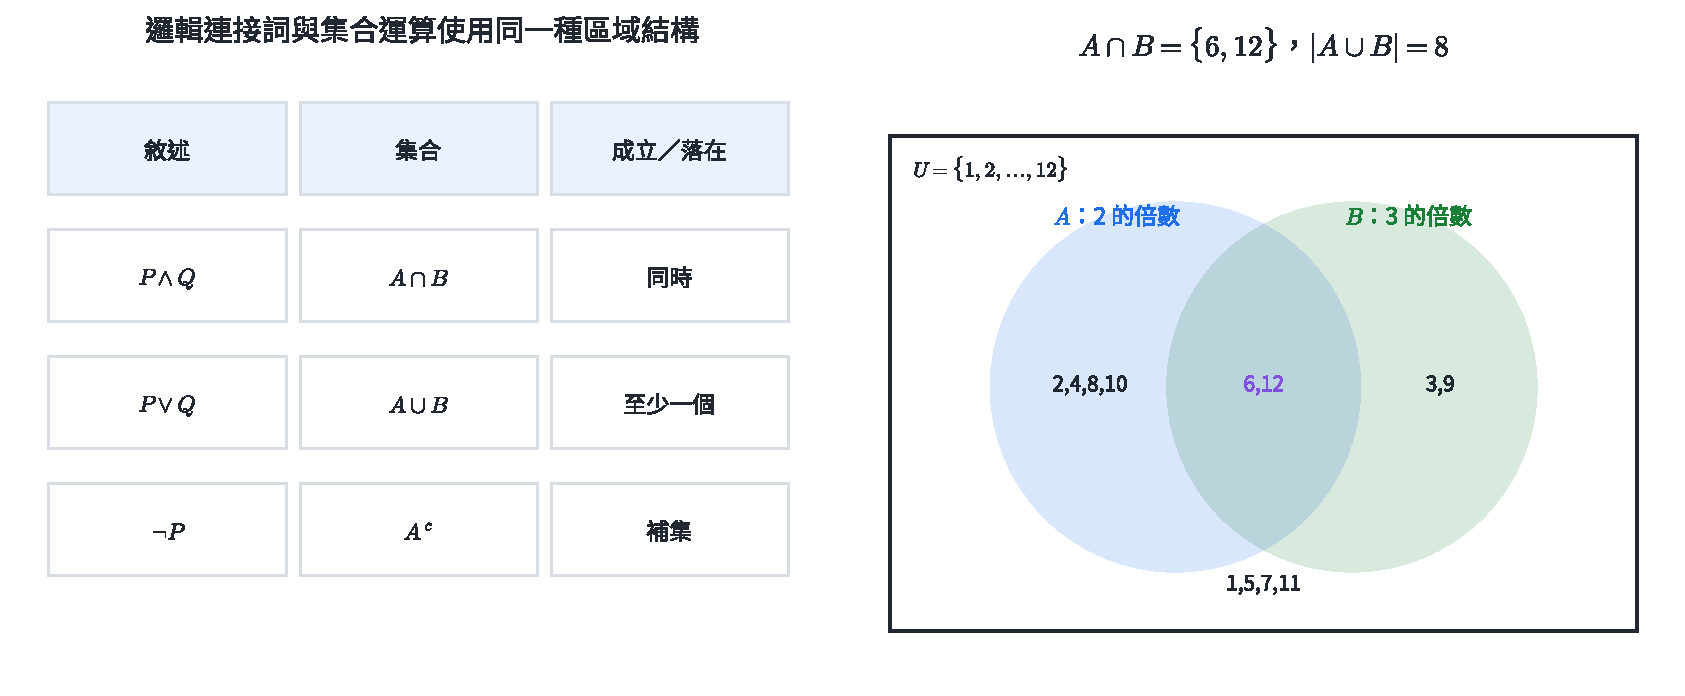
\includegraphics[width=0.96\linewidth,height=\textheight,keepaspectratio,alt={邏輯連接詞與集合運算使用相同的區域結構}]{assets/數2-3-邏輯與集合運算.pdf}
\caption{邏輯連接詞與集合運算使用相同的區域結構}
\end{figure}

以任意元素 \(x\) 檢查，

\[
x\in(A\cap B)^c
\Leftrightarrow x\notin A\cap B
\Leftrightarrow (x\notin A)\text{ 或 }(x\notin B),
\]

因此

\[
(A\cap B)^c=A^c\cup B^c.
\]

同理可得 \((A\cup B)^c=A^c\cap B^c\)。這就是集合的笛摩根律。

\subsection{例 1｜判斷充分條件與必要條件}\label{ux4f8b-1ux5224ux65b7ux5145ux5206ux689dux4ef6ux8207ux5fc5ux8981ux689dux4ef6}

討論範圍是整數。令

\[
P:\ x\text{ 是 }6\text{ 的倍數},\qquad
Q:\ x\text{ 是 }3\text{ 的倍數}.
\]

若 \(P\) 成立，可寫成 \(x=6k=3(2k)\)，所以 \(Q\) 成立，即 \(P\Rightarrow Q\)。

\(x=3\) 符合 \(Q\)，但不符合 \(P\)，所以 \(Q\Rightarrow P\) 不成立。因此 \(P\) 是 \(Q\) 的充分條件，\(Q\) 是 \(P\) 的必要條件。

\subsection{例 2｜由全集計算交集、聯集與補集}\label{ux4f8b-2ux7531ux5168ux96c6ux8a08ux7b97ux4ea4ux96c6ux806fux96c6ux8207ux88dcux96c6}

令 \(U=\{1,2,\ldots,12\}\)，\(A\) 是 \(2\) 的倍數所成集合，\(B\) 是 \(3\) 的倍數所成集合。則

\[
A=\{2,4,6,8,10,12\},\qquad B=\{3,6,9,12\}.
\]

所以

\[
A\cap B=\{6,12\},
\]

\[
A\cup B=\{2,3,4,6,8,9,10,12\},
\]

\[
(A\cup B)^c=\{1,5,7,11\}.
\]

再直接計算 \(A^c\cap B^c\)，也得到 \(\{1,5,7,11\}\)，與笛摩根律一致。

\subsection{1.3 分節練習}\label{ux5206ux7bc0ux7df4ux7fd2}

\begin{enumerate}
\def\labelenumi{\arabic{enumi}.}
\tightlist
\item
  判斷「\(2+5=8\)」與「請把門關上」是否為命題；若是命題，寫出真假。
\item
  討論範圍為整數。令 \(P:x\) 是 \(12\) 的倍數，\(Q:x\) 是 \(4\) 的倍數。判斷 \(P\Rightarrow Q\) 與 \(Q\Rightarrow P\)，並說明充分、必要關係。
\item
  寫出命題「\(x>1\) 且 \(x\le5\)」的否定。
\item
  令 \(U=\{1,2,\ldots,10\}\)，\(A=\{1,2,3,4,5\}\)，\(B=\{2,4,6,8,10\}\)。求 \(A\cap B\)、\(A\cup B\)、\(A-B\) 與 \(B^c\)。
\item
  用元素是否屬於集合的方式，證明 \((A\cup B)^c=A^c\cap B^c\)。
\end{enumerate}

\subsection{1.4 分節練習解析}\label{ux5206ux7bc0ux7df4ux7fd2ux89e3ux6790}

\begin{enumerate}
\def\labelenumi{\arabic{enumi}.}
\tightlist
\item
  「\(2+5=8\)」可判定真假，是假命題；「請把門關上」是指令，沒有真值，因此不屬於命題。
\item
  \(x=12k=4(3k)\)，故 \(P\Rightarrow Q\) 成立。\(x=4\) 符合 \(Q\) 而不符合 \(P\)，故 \(Q\Rightarrow P\) 不成立。\(P\) 是 \(Q\) 的充分條件，\(Q\) 是 \(P\) 的必要條件。
\item
  原命題是 \(P\wedge Q\)，其中 \(P:x>1\)、\(Q:x\le5\)。由笛摩根律，否定為 \(x\le1\) 或 \(x>5\)。
\item
  \(A\cap B=\{2,4\}\)；\(A\cup B=\{1,2,3,4,5,6,8,10\}\)；\(A-B=\{1,3,5\}\)；\(B^c=\{1,3,5,7,9\}\)。
\item
  對任意 \(x\in U\)，\(x\in(A\cup B)^c\) 等價於 \(x\notin A\cup B\)，也等價於 \(x\notin A\) 且 \(x\notin B\)，最後等價於 \(x\in A^c\cap B^c\)。兩集合含有完全相同的元素，所以相等。
\end{enumerate}

邏輯規則可用來整理搜尋條件、電路條件與程式判斷；集合運算則把條件轉成可視化區域，後續計數與事件機率都直接沿用這套語言。

\section{2. 基本計數原理}\label{ux57faux672cux8a08ux6578ux539fux7406}

\subsection{2.1 加法原理與乘法原理}\label{ux52a0ux6cd5ux539fux7406ux8207ux4e58ux6cd5ux539fux7406}

若一個任務可由互不重疊的甲類或乙類完成，甲類有 \(m\) 種、乙類有 \(n\) 種，總數為 \(m+n\)。這是\textbf{加法原理}。類別互斥可確保每個結果只被計算一次。

若一個任務依序完成兩個步驟，第一步有 \(m\) 種，而且第一步每種選擇之後，第二步都有 \(n\) 種，總數為 \(m\times n\)。這是\textbf{乘法原理}。多步驟情況可繼續相乘；樹狀圖的每一條根到葉路徑對應一個完整結果。

\begin{figure}
\centering
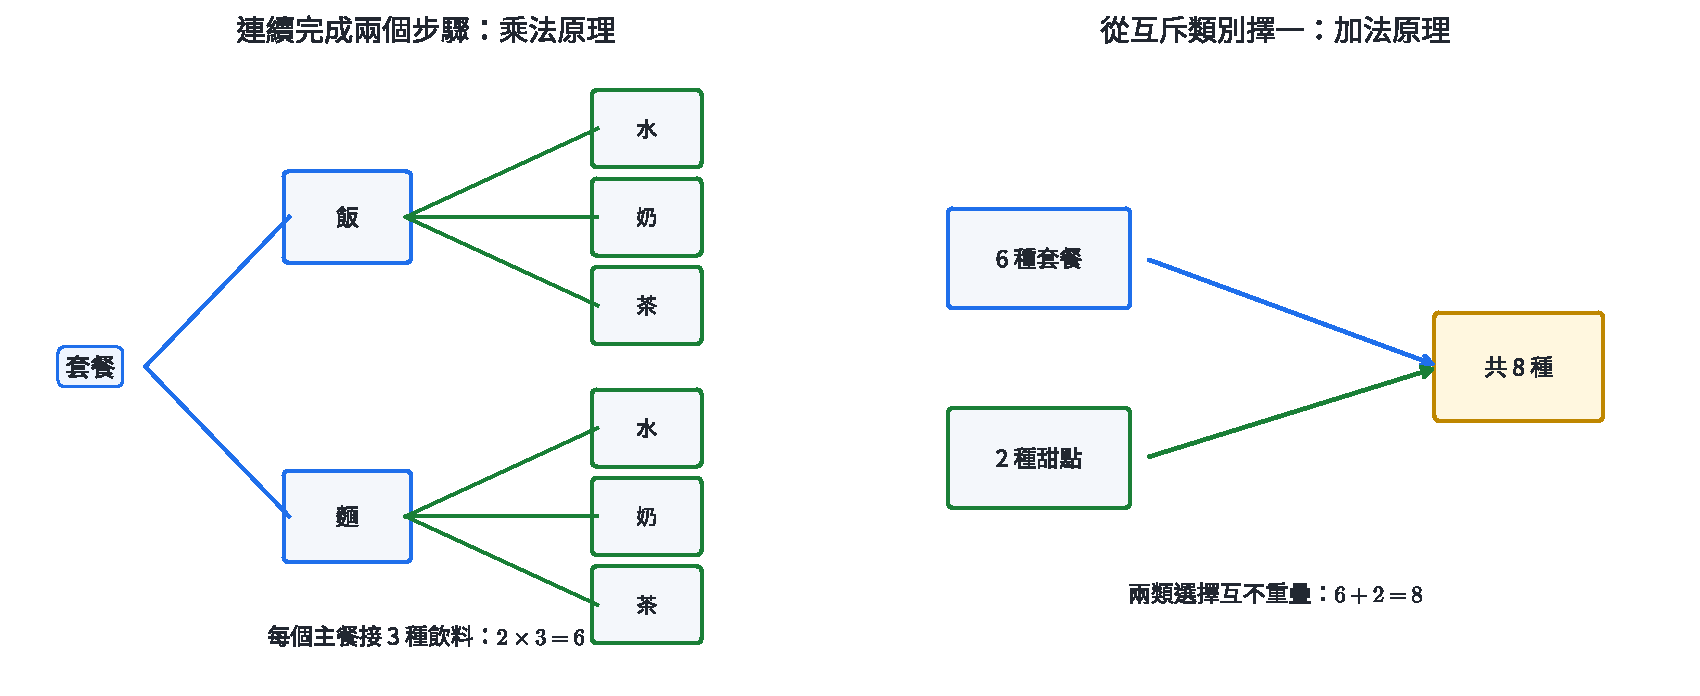
\includegraphics[width=0.96\linewidth,height=\textheight,keepaspectratio,alt={樹狀圖的葉節點呈現乘法原理，互斥類別的合併呈現加法原理}]{assets/數2-3-加法乘法樹.pdf}
\caption{樹狀圖的葉節點呈現乘法原理，互斥類別的合併呈現加法原理}
\end{figure}

\subsection{2.2 取捨原理}\label{ux53d6ux6368ux539fux7406}

當兩個類別有重疊時，\(|A|+|B|\) 會把 \(A\cap B\) 算兩次，因此聯集個數是

\[
\boxed{|A\cup B|=|A|+|B|-|A\cap B|}.
\]

三集合的公式依同樣原理修正重複次數：

\[
|A\cup B\cup C|=|A|+|B|+|C|-|A\cap B|-|A\cap C|-|B\cap C|+|A\cap B\cap C|.
\]

三重交集一開始被加三次，接著在三個兩兩交集中被減三次，因此最後補加一次。

\begin{figure}
\centering
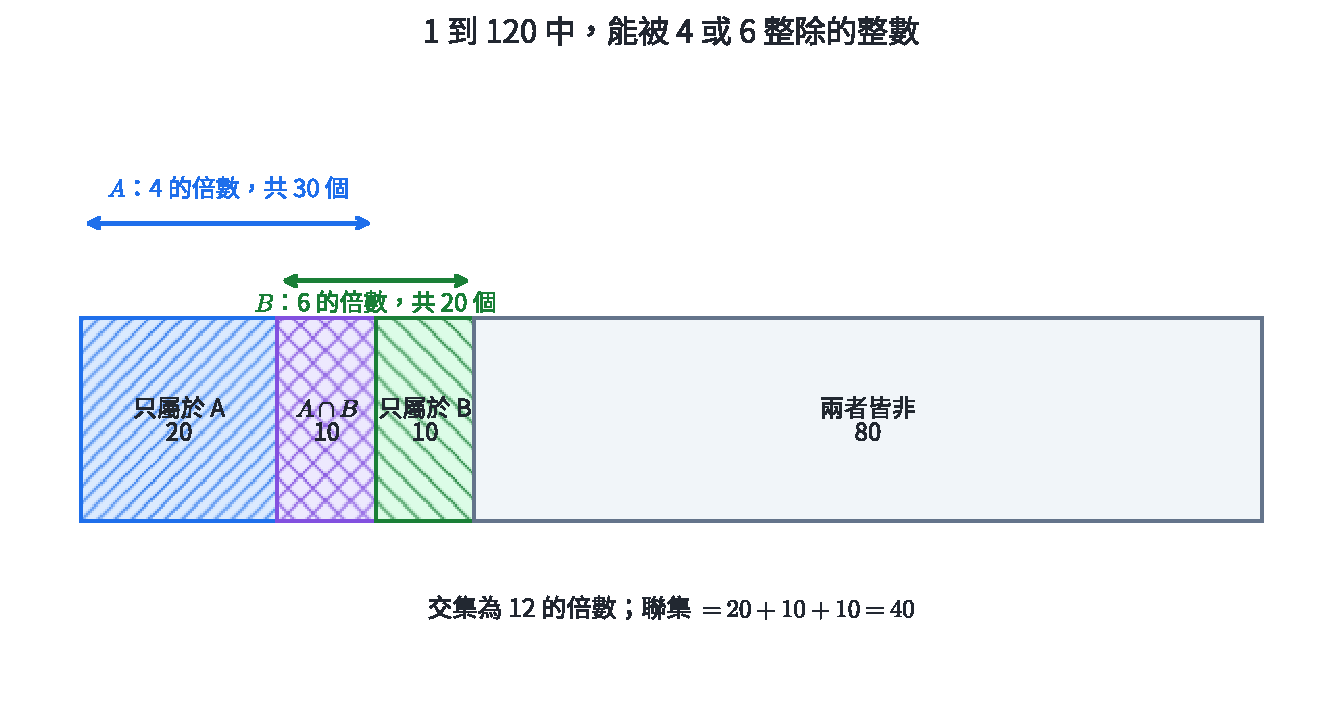
\includegraphics[width=0.88\linewidth,height=\textheight,keepaspectratio,alt={交集先被兩集合各算一次，因此聯集要減去一次交集}]{assets/數2-3-取捨原理.pdf}
\caption{交集先被兩集合各算一次，因此聯集要減去一次交集}
\end{figure}

\subsection{例 3｜分步形成代碼}\label{ux4f8b-3ux5206ux6b65ux5f62ux6210ux4ee3ux78bc}

一組代碼依序由 2 個英文字母與 3 個數字構成，字母與數字都可重複。五個位置依序有 \(26,26,10,10,10\) 種選擇。由乘法原理，總數是

\[
26^2\cdot10^3=676000.
\]

\subsection{例 4｜用取捨原理修正重複計數}\label{ux4f8b-4ux7528ux53d6ux6368ux539fux7406ux4feeux6b63ux91cdux8907ux8a08ux6578}

在 \(1\) 到 \(120\) 的整數中，能被 \(4\) 或 \(6\) 整除的共有幾個？

能被 \(4\) 整除的有 \(\lfloor120/4\rfloor=30\) 個；能被 \(6\) 整除的有 \(20\) 個。兩者同時成立就是 \(12\) 的倍數，共 \(10\) 個。因此

\[
30+20-10=40.
\]

\subsection{2.3 分節練習}\label{ux5206ux7bc0ux7df4ux7fd2-1}

\begin{enumerate}
\def\labelenumi{\arabic{enumi}.}
\tightlist
\item
  一家店有 4 種飯、3 種麵與 2 種沙拉。只選一份主餐，共有幾種選法？
\item
  從甲地到乙地有 3 條道路，從乙地到丙地有 5 條道路。經乙地由甲到丙共有幾條路線？
\item
  一個帳號識別碼由 1 個大寫字母與 4 個數字構成，可重複。共有幾個識別碼？
\item
  \(1\) 到 \(200\) 中，能被 \(5\) 或 \(8\) 整除的整數有幾個？
\item
  某班 40 人中，會游泳的有 24 人，會騎自行車的有 31 人，兩者都會的有 20 人。至少會一項與兩項都不會的各有幾人？
\item
  從 \(A\) 到 \(B\) 有 2 種交通方式，從 \(B\) 到 \(C\) 有 3 種；另有 4 種可由 \(A\) 直達 \(C\)。計算由 \(A\) 到 \(C\) 的方式數。
\end{enumerate}

\subsection{2.4 分節練習解析}\label{ux5206ux7bc0ux7df4ux7fd2ux89e3ux6790-1}

\begin{enumerate}
\def\labelenumi{\arabic{enumi}.}
\tightlist
\item
  三類互斥，使用加法原理：\(4+3+2=9\) 種。
\item
  每條甲乙道路都可接 5 條乙丙道路，使用乘法原理：\(3\times5=15\) 條。
\item
  五個位置的選擇數是 \(26,10,10,10,10\)，故共有 \(26\times10^4=260000\) 個。
\item
  \(5\) 的倍數有 \(40\) 個，\(8\) 的倍數有 \(25\) 個，兩者交集是 \(40\) 的倍數，共 \(5\) 個。答案為 \(40+25-5=60\) 個。
\item
  至少會一項的人數是 \(24+31-20=35\)；兩項都不會是 \(40-35=5\) 人。
\item
  經 \(B\) 的路線有 \(2\times3=6\) 種；直達與經 \(B\) 是互斥類別，所以總數 \(6+4=10\) 種。
\end{enumerate}

計數原理常用於密碼空間、實驗組合、流程分支與資料庫查詢。建立模型時，先說明類別是否互斥、步驟是否都要完成，再決定相加或相乘。

\section{3. 排列}\label{ux6392ux5217}

\subsection{3.1 階乘與相異物排列}\label{ux968eux4e58ux8207ux76f8ux7570ux7269ux6392ux5217}

\(n\) 個相異物件排成一列：第一個位置有 \(n\) 種選擇，第二個位置剩 \(n-1\) 種，依序到最後一個位置只有 \(1\) 種，因此排列數為

\[
n!=n(n-1)\cdots2\cdot1.
\]

定義 \(0!=1\)，可讓後續公式在邊界情況保持一致。

從 \(n\) 個相異物件選出 \(r\) 個並依序排列，前 \(r\) 個位置的選擇數依序為 \(n,n-1,\ldots,n-r+1\)，所以

\[
\boxed{P^n_r=n(n-1)\cdots(n-r+1)=\frac{n!}{(n-r)!}},
\qquad 0\le r\le n.
\]

排列模型中的職務、名次、座位或讀取順序都會區分結果。例如「甲任主席、乙任副主席」與「乙任主席、甲任副主席」是兩個結果。

\subsection{3.2 條件排列的三種結構}\label{ux689dux4ef6ux6392ux5217ux7684ux4e09ux7a2eux7d50ux69cb}

\begin{itemize}
\tightlist
\item
  \textbf{固定或指定位置}：先處理指定位置，再排剩餘物件。
\item
  \textbf{相鄰成塊}：把必須相鄰的物件先視為一個整體，最後乘上塊內排列數。
\item
  \textbf{分隔空隙}：先排一類物件，再從其前後空隙放入另一類，可直接保證分隔條件。
\end{itemize}

\begin{figure}
\centering
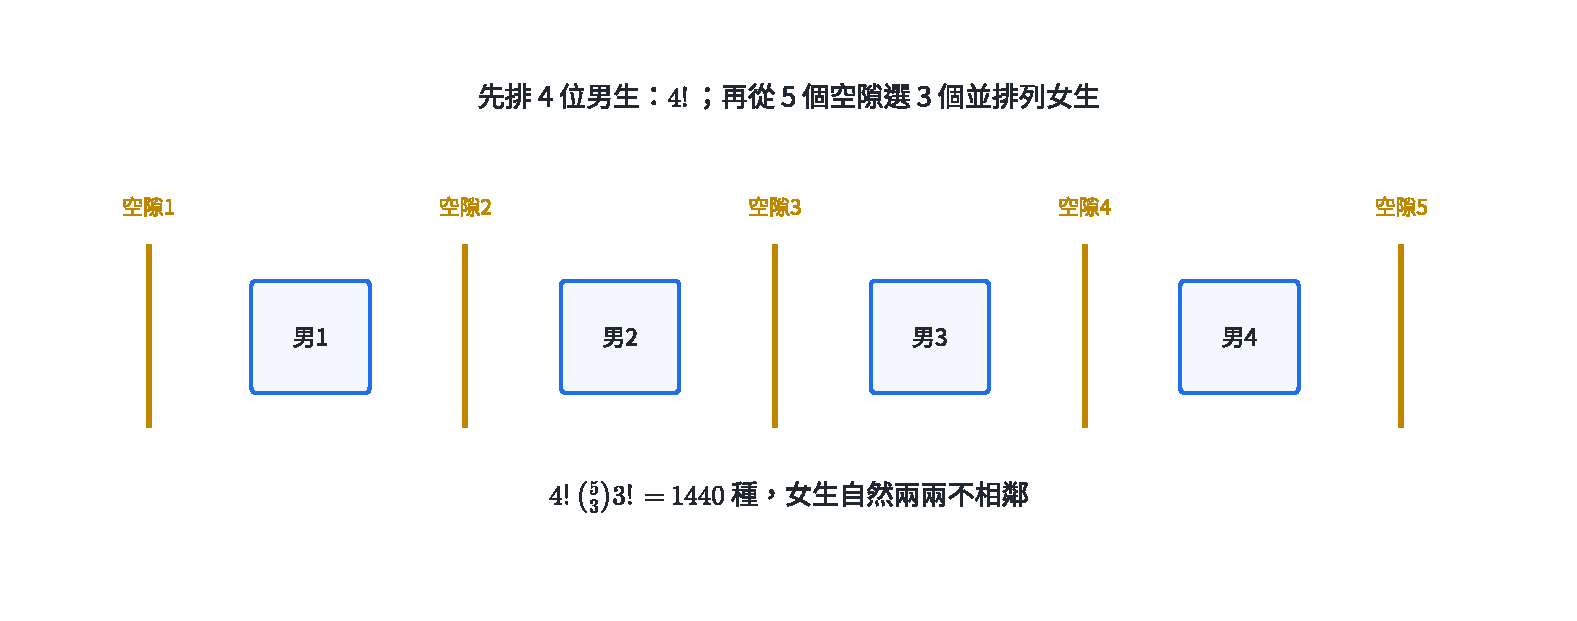
\includegraphics[width=0.94\linewidth,height=\textheight,keepaspectratio,alt={先排一類物件形成空隙，再選空隙放入另一類}]{assets/數2-3-排列位置與空隙.pdf}
\caption{先排一類物件形成空隙，再選空隙放入另一類}
\end{figure}

\subsection{3.3 含相同物件的排列}\label{ux542bux76f8ux540cux7269ux4ef6ux7684ux6392ux5217}

若 \(n\) 個位置中有 \(m_1\) 個物件彼此相同、\(m_2\) 個物件彼此相同，且 \(m_1+m_2+\cdots+m_k=n\)，暫時替同類物件加上編號會得到 \(n!\) 個排列。每個實際結果都因同類物件內部交換而重複 \(m_1!m_2!\cdots m_k!\) 次，因此不同排列數為

\[
\boxed{\frac{n!}{m_1!m_2!\cdots m_k!}}.
\]

方格最短路徑也是同一模型：若一定要向右 \(a\) 步、向上 \(b\) 步，每條最短路徑就是 \(a\) 個相同的 R 與 \(b\) 個相同的 U 的排列，路徑數為

\[
\frac{(a+b)!}{a!b!}.
\]

\begin{figure}
\centering
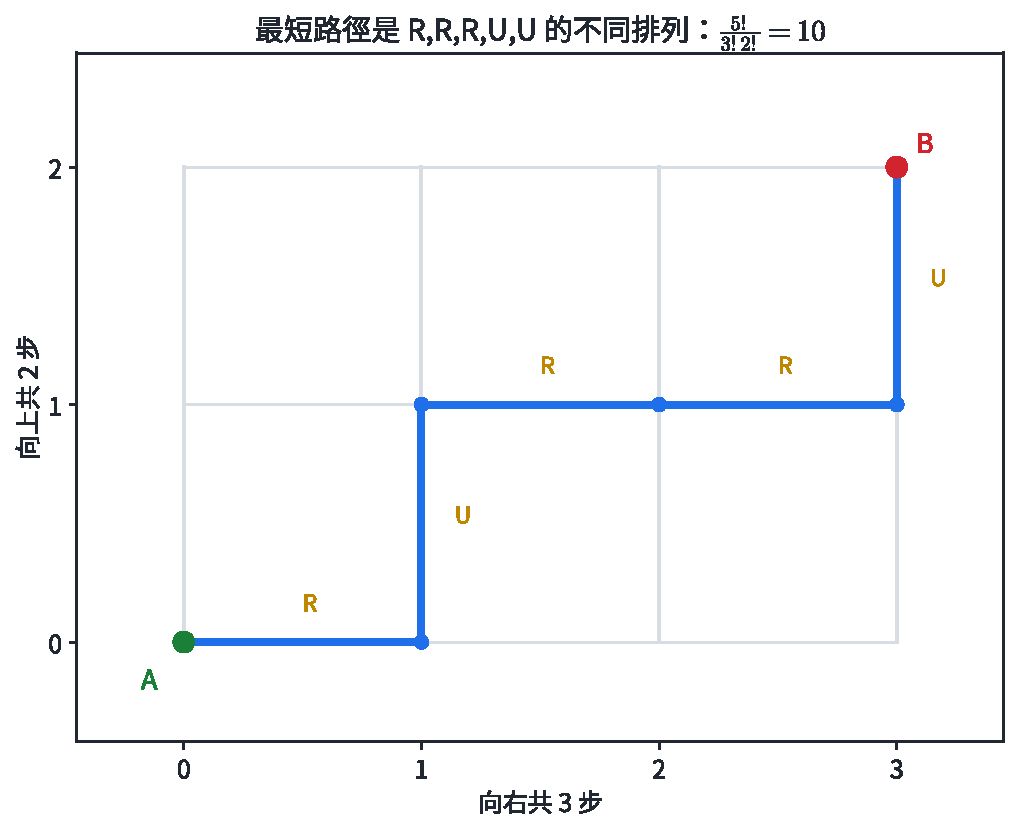
\includegraphics[width=0.8\linewidth,height=\textheight,keepaspectratio,alt={從 A 到 B 的最短路徑等同於三個 R 與兩個 U 的排列}]{assets/數2-3-相同物最短路.pdf}
\caption{從 A 到 B 的最短路徑等同於三個 R 與兩個 U 的排列}
\end{figure}

\subsection{例 5｜選人擔任有次序的職務}\label{ux4f8b-5ux9078ux4ebaux64d4ux4efbux6709ux6b21ux5e8fux7684ux8077ux52d9}

7 人中選出 4 人，依序擔任主席、副主席、紀錄與司儀，共有幾種安排？

四個職務依序有 \(7,6,5,4\) 種選擇，因此

\[
P^7_4=7\cdot6\cdot5\cdot4=840.
\]

\subsection{例 6｜相鄰條件用成塊與補集計算}\label{ux4f8b-6ux76f8ux9130ux689dux4ef6ux7528ux6210ux584aux8207ux88dcux96c6ux8a08ux7b97}

甲、乙等 6 人排成一列。求甲乙相鄰與不相鄰的排列數。

甲乙相鄰時，把兩人視為一塊，連同其餘 4 人共有 5 個單位。單位可排 \(5!\) 種，塊內有甲乙、乙甲兩種，所以

\[
5!\cdot2!=240.
\]

全部排列有 \(6!=720\) 種，因此甲乙不相鄰有

\[
720-240=480
\]

種。

\subsection{例 7｜相同字母排列}\label{ux4f8b-7ux76f8ux540cux5b57ux6bcdux6392ux5217}

單字 BANANA 的 6 個字母共有幾種不同排列？

A 有 3 個、N 有 2 個、B 有 1 個，所以

\[
\frac{6!}{3!2!}=\frac{720}{12}=60.
\]

\subsection{例 8｜格點最短路徑}\label{ux4f8b-8ux683cux9edeux6700ux77edux8defux5f91}

從 \((0,0)\) 走到 \((4,3)\)，每步只能向右或向上。最短路徑共有幾條？

每條最短路徑必含 4 個 R 與 3 個 U，共 7 步。不同路徑數為

\[
\frac{7!}{4!3!}=\binom{7}{3}=35.
\]

\subsection{3.4 分節練習}\label{ux5206ux7bc0ux7df4ux7fd2-2}

\begin{enumerate}
\def\labelenumi{\arabic{enumi}.}
\tightlist
\item
  計算 \(P^9_3\)。
\item
  8 位選手中選出金、銀、銅牌得主，共有幾種結果？
\item
  甲、乙、丙、丁、戊排成一列，甲固定在最左端，共有幾種排法？
\item
  7 人排成一列，甲、乙、丙三人必須相鄰，共有幾種排法？
\item
  MISS 的 4 個字母共有幾種不同排列？
\item
  從 \((0,0)\) 到 \((5,2)\)，每步只能向右或向上，共有幾條最短路徑？
\end{enumerate}

\subsection{3.5 分節練習解析}\label{ux5206ux7bc0ux7df4ux7fd2ux89e3ux6790-2}

\begin{enumerate}
\def\labelenumi{\arabic{enumi}.}
\tightlist
\item
  \(P^9_3=9\cdot8\cdot7=504\)。
\item
  三面獎牌有次序，故為 \(P^8_3=8\cdot7\cdot6=336\) 種。
\item
  甲的位置已固定，其餘 4 人排列，有 \(4!=24\) 種。
\item
  把甲乙丙視為一塊，連同其餘 4 人共有 5 個單位，外部有 \(5!\) 種；塊內有 \(3!\) 種。答案為 \(5!3!=720\) 種。
\item
  S 有 2 個，因此不同排列數為 \(4!/2!=12\)。
\item
  最短路徑含 5 個 R 與 2 個 U，共 \(7!/(5!2!)=21\) 條。
\end{enumerate}

排列可描述工作排程、資料讀取次序、座位與路由。限制條件會改變結果空間的結構；固定位置、成塊、空隙與補集是把條件直接轉成計數步驟的方法。

\section{4. 重複排列}\label{ux91cdux8907ux6392ux5217}

\subsection{4.1 每個位置可重複選擇}\label{ux6bcfux500bux4f4dux7f6eux53efux91cdux8907ux9078ux64c7}

用 \(n\) 種符號填入 \(r\) 個有次序的位置，而且每個符號可重複使用。每一個位置都有 \(n\) 種選擇，由乘法原理共有

\[
\boxed{n^r}
\]

種。這類型也稱為可重複取用的排列；重點是位置有順序、每次選擇後可再次使用同一符號。

若相鄰位置需使用不同符號，第一個位置有 \(n\) 種，之後每個位置都排除前一格使用的符號，因此共有

\[
n(n-1)^{r-1}
\]

種。

\subsection{例 9｜可重複的符號序列}\label{ux4f8b-9ux53efux91cdux8907ux7684ux7b26ux865fux5e8fux5217}

以 A、B、C、D 四種符號形成長度 6 的序列，符號可重複，共有幾種？

六個位置各有 4 種選擇，所以

\[
4^6=4096.
\]

\subsection{例 10｜相鄰色塊使用不同顏色}\label{ux4f8b-10ux76f8ux9130ux8272ux584aux4f7fux7528ux4e0dux540cux984fux8272}

用 7 種顏色塗 4 個排成一列的色塊，相鄰色塊顏色不同，共有幾種？

第一格有 7 種。第二格到第四格各有 6 種，因為只需避開緊鄰前一格的顏色。因此

\[
7\cdot6^3=1512.
\]

\subsection{4.2 分節練習}\label{ux5206ux7bc0ux7df4ux7fd2-3}

\begin{enumerate}
\def\labelenumi{\arabic{enumi}.}
\tightlist
\item
  用數字 \(0,1,2\) 形成長度 5 的字串，可重複，共有幾個？
\item
  一份 8 題的是非題，每題作答「是」或「否」，共有幾種完整作答方式？
\item
  5 件不同工作各分配給甲、乙、丙三人中的一人，每人可分到多件或零件，共有幾種分配？
\item
  用 5 種顏色塗 6 個排成一列的色塊，相鄰色塊顏色不同，共有幾種？
\item
  一個長度 7 的二進位字串中，第一位固定為 1，其餘位置可任取 0 或 1，共有幾個？
\end{enumerate}

\subsection{4.3 分節練習解析}\label{ux5206ux7bc0ux7df4ux7fd2ux89e3ux6790-3}

\begin{enumerate}
\def\labelenumi{\arabic{enumi}.}
\tightlist
\item
  五個位置各有 3 種選擇，所以共有 \(3^5=243\) 個。
\item
  八題各有 2 種選擇，共 \(2^8=256\) 種。
\item
  對每一件工作，可選甲、乙或丙，共 \(3^5=243\) 種。這裡以工作為有標記的位置。
\item
  第一格 5 種，後五格各 4 種，共 \(5\cdot4^5=5120\) 種。
\item
  第一位已固定，剩餘 6 位各有 2 種，所以有 \(2^6=64\) 個。
\end{enumerate}

重複排列用於密碼、DNA 序列、問卷作答、通訊符號與工作分派。位置代表的欄位必須清楚；若某些位置受前一位置限制，就逐步更新該位置的可選數。

\section{5. 組合}\label{ux7d44ux5408}

\subsection{5.1 選取而不排序}\label{ux9078ux53d6ux800cux4e0dux6392ux5e8f}

從 \(n\) 個相異物件中選出 \(r\) 個，只記錄被選成員而不區分先後，稱為\textbf{組合}，組合數記作 \(\binom{n}{r}\) 或 \(C^n_r\)。

先把選出的 \(r\) 個物件排成有次序的結果，共有 \(P^n_r\) 種。每一個無序小組在這些排列中恰好出現 \(r!\) 次，因此

\[
P^n_r=\binom{n}{r}r!,
\]

\[
\boxed{\binom{n}{r}=\frac{n!}{r!(n-r)!}},
\qquad 0\le r\le n.
\]

\begin{figure}
\centering
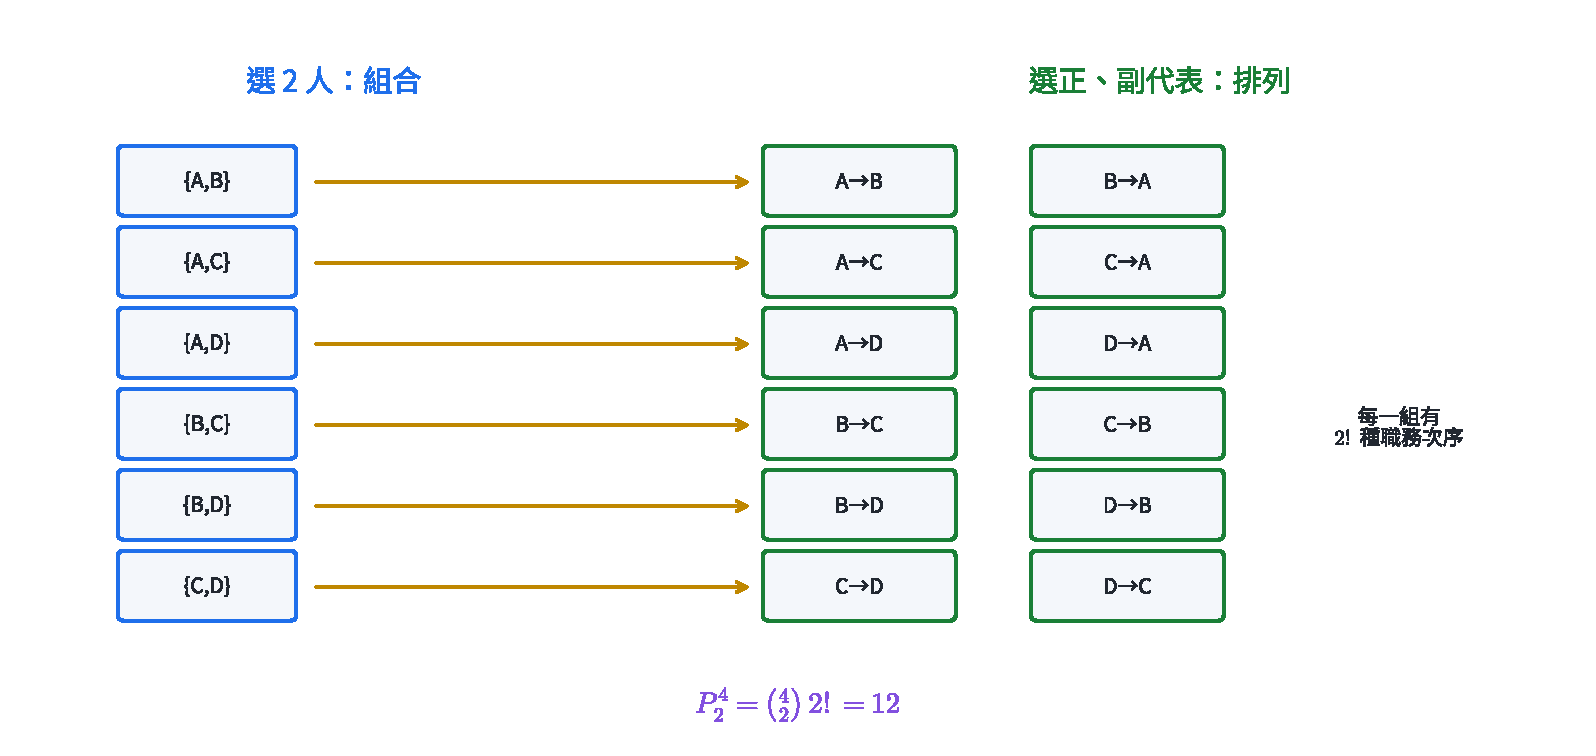
\includegraphics[width=0.94\linewidth,height=\textheight,keepaspectratio,alt={每個兩人小組對應兩種有職務次序的排列}]{assets/數2-3-排列與組合比較.pdf}
\caption{每個兩人小組對應兩種有職務次序的排列}
\end{figure}

選出 \(r\) 人等同於決定留下的 \(n-r\) 人，所以

\[
\boxed{\binom{n}{r}=\binom{n}{n-r}}.
\]

邊界情況是 \(\binom{n}{0}=\binom{n}{n}=1\)：選空集合與選出全部各只有一種方式。

\subsection{5.2 條件選取與分組}\label{ux689dux4ef6ux9078ux53d6ux8207ux5206ux7d44}

含條件的組合題通常先依「選了幾個特定類別」分成互斥情況，再把各情況相加。若把相異物件分成數個群組，可依序選出各組；當兩個群組大小相同且沒有名稱時，交換兩組不產生新結果，因此還要除去相同群組的交換次數。

例如 8 本相異書分成大小 \(4,2,2\) 的三堆，其中兩個 2 本堆沒有標籤。先選 4 本，再從剩下 4 本選 2 本會得到

\[
\binom84\binom42\binom22,
\]

但兩個 2 本堆可互換，所以實際分法為

\[
\frac{\binom84\binom42\binom22}{2!}.
\]

\subsection{例 11｜選出委員}\label{ux4f8b-11ux9078ux51faux59d4ux54e1}

10 人中選 4 人組成委員會，共有幾種？

委員之間沒有職務差別，使用組合：

\[
\binom{10}{4}=\frac{10!}{4!6!}=210.
\]

\subsection{例 12｜至少條件用互斥分類}\label{ux4f8b-12ux81f3ux5c11ux689dux4ef6ux7528ux4e92ux65a5ux5206ux985e}

5 位男生與 4 位女生中選 4 人，至少有 2 位女生，共有幾種？

依女生人數分成 2、3、4 人三類：

\[
\binom42\binom52+\binom43\binom51+\binom44\binom50
=6\cdot10+4\cdot5+1=81.
\]

三類的女生人數不同，彼此互斥，可直接相加。

\subsection{例 13｜分成沒有名稱的等大群組}\label{ux4f8b-13ux5206ux6210ux6c92ux6709ux540dux7a31ux7684ux7b49ux5927ux7fa4ux7d44}

6 支相異鉛筆平均分成 3 組，每組 2 支，群組沒有名稱。共有幾種分法？

依序選三組會得到

\[
\binom62\binom42\binom22.
\]

同一分組會因三組的先後次序被計算 \(3!\) 次，因此

\[
\frac{\binom62\binom42\binom22}{3!}
=\frac{15\cdot6}{6}=15.
\]

\subsection{5.3 分節練習}\label{ux5206ux7bc0ux7df4ux7fd2-4}

\begin{enumerate}
\def\labelenumi{\arabic{enumi}.}
\tightlist
\item
  計算 \(\binom{12}{3}\) 與 \(\binom{12}{9}\)。
\item
  9 本不同的書中選 5 本帶出門，共有幾種選法？
\item
  平面上有 8 點，其中任三點不共線。可決定多少條直線？
\item
  6 位男生、5 位女生中選 4 人，恰有 2 位女生，共有幾種？
\item
  7 人中選 3 人，甲與乙恰有一人入選，共有幾種？
\item
  8 個相異物件分成兩組，每組 4 個，兩組沒有名稱，共有幾種分法？
\end{enumerate}

\subsection{5.4 分節練習解析}\label{ux5206ux7bc0ux7df4ux7fd2ux89e3ux6790-4}

\begin{enumerate}
\def\labelenumi{\arabic{enumi}.}
\tightlist
\item
  \(\binom{12}{3}=12\cdot11\cdot10/(3\cdot2\cdot1)=220\)。由對稱性，\(\binom{12}{9}=\binom{12}{3}=220\)。
\item
  只記錄選到哪 5 本，故有 \(\binom95=126\) 種。
\item
  每兩點決定一條直線，任三點不共線確保不同點對得到不同直線，因此有 \(\binom82=28\) 條。
\item
  選 2 位女生與 2 位男生：\(\binom52\binom62=10\cdot15=150\) 種。
\item
  先從甲乙中選 1 人，有 \(\binom21\) 種；再從其餘 5 人選 2 人，有 \(\binom52\) 種。答案 \(2\cdot10=20\) 種。
\item
  先選第一組有 \(\binom84=70\) 種，但同一分組因兩組交換而重複 2 次，故有 \(70/2=35\) 種。
\end{enumerate}

組合用於抽樣、委員會、資料特徵選取與幾何物件計數。判斷標準是交換選取順序後，結果的身分是否改變；若群組或職務有名稱，就保留相應次序。

\section{6. 二項式定理}\label{ux4e8cux9805ux5f0fux5b9aux7406}

\subsection{6.1 係數來自選擇因子}\label{ux4fc2ux6578ux4f86ux81eaux9078ux64c7ux56e0ux5b50}

把 \((x+y)^n\) 寫成 \(n\) 個因子的乘積：

\[
(x+y)^n=(x+y)(x+y)\cdots(x+y).
\]

要形成 \(x^{n-k}y^k\)，必須從 \(n\) 個因子中選出 \(k\) 個提供 \(y\)，其餘提供 \(x\)。選法有 \(\binom nk\) 種，所以

\[
\boxed{(x+y)^n=\sum_{k=0}^{n}\binom nk x^{n-k}y^k}.
\]

第 \(k+1\) 項是

\[
T_{k+1}=\binom nk x^{n-k}y^k.
\]

\begin{figure}
\centering
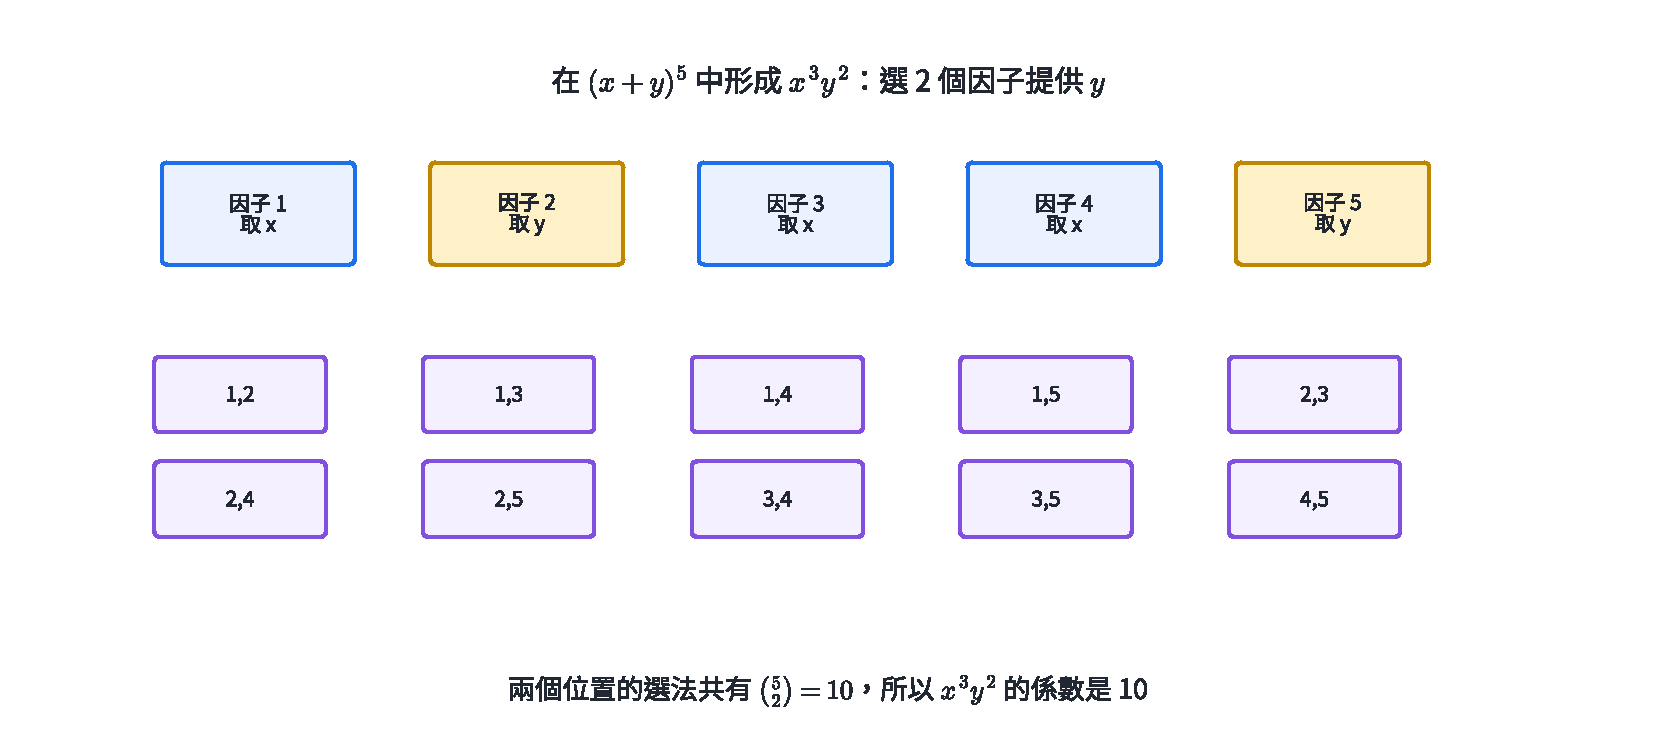
\includegraphics[width=0.95\linewidth,height=\textheight,keepaspectratio,alt={在五個因子中選兩個提供 y，形成 x 三次方 y 二次方}]{assets/數2-3-二項式選因子.pdf}
\caption{在五個因子中選兩個提供 y，形成 x 三次方 y 二次方}
\end{figure}

若因子是 \((ax+b)^n\)，通項改為

\[
T_{k+1}=\binom nk (ax)^{n-k}b^k.
\]

負號、係數與變數次方都留在被選的項中一起乘入。

\subsection{例 14｜求指定項的係數}\label{ux4f8b-14ux6c42ux6307ux5b9aux9805ux7684ux4fc2ux6578}

求 \((2x-y)^5\) 中 \(x^3y^2\) 的係數。

要得到 \(y^2\)，選 \(k=2\)；其餘三個因子提供 \(2x\)。對應項為

\[
\binom52(2x)^3(-y)^2
=10\cdot8x^3y^2.
\]

所以係數是

\[
\boxed{80}.
\]

\subsection{例 15｜利用次方條件找常數項}\label{ux4f8b-15ux5229ux7528ux6b21ux65b9ux689dux4ef6ux627eux5e38ux6578ux9805}

求 \(\left(x^2+\dfrac1x\right)^6\) 的常數項。

通項為

\[
\binom6k(x^2)^{6-k}\left(\frac1x\right)^k
=\binom6k x^{12-3k}.
\]

常數項的指數為 \(0\)，所以

\[
12-3k=0\quad\Longrightarrow\quad k=4.
\]

常數項是

\[
\binom64=15.
\]

\subsection{6.2 分節練習}\label{ux5206ux7bc0ux7df4ux7fd2-5}

\begin{enumerate}
\def\labelenumi{\arabic{enumi}.}
\tightlist
\item
  展開 \((x+y)^4\)。
\item
  求 \((3x+2)^5\) 中 \(x^3\) 的係數。
\item
  求 \((x-2y)^6\) 中 \(x^4y^2\) 的係數。
\item
  求 \(\left(x+\dfrac1x\right)^8\) 的常數項。
\item
  求 \((1+2x)^7\) 中 \(x^5\) 的係數。
\end{enumerate}

\subsection{6.3 分節練習解析}\label{ux5206ux7bc0ux7df4ux7fd2ux89e3ux6790-5}

\begin{enumerate}
\def\labelenumi{\arabic{enumi}.}
\tightlist
\item
  係數依序為 \(1,4,6,4,1\)，故 \((x+y)^4=x^4+4x^3y+6x^2y^2+4xy^3+y^4\)。
\item
  \(x^3\) 表示 3 個因子提供 \(3x\)、2 個提供 \(2\)，係數為 \(\binom53 3^3 2^2=10\cdot27\cdot4=1080\)。
\item
  選 2 個因子提供 \(-2y\)，係數為 \(\binom62(-2)^2=15\cdot4=60\)。
\item
  通項為 \(\binom8k x^{8-2k}\)。令 \(8-2k=0\) 得 \(k=4\)，常數項為 \(\binom84=70\)。
\item
  選 5 個因子提供 \(2x\)，係數為 \(\binom75 2^5=21\cdot32=672\)。
\end{enumerate}

二項式定理可快速取得多項式係數，也可用於近似計算、機率分布與組合恆等式。通項把「選哪些因子」與「所得次方」連起來，因而能直接定位指定項。

\section{7. 巴斯卡三角形}\label{ux5df4ux65afux5361ux4e09ux89d2ux5f62}

\subsection{7.1 相鄰兩數相加的原因}\label{ux76f8ux9130ux5169ux6578ux76f8ux52a0ux7684ux539fux56e0}

巴斯卡三角形第 \(n\) 列依序放入

\[
\binom n0,\binom n1,\ldots,\binom nn.
\]

固定一個特別元素 \(a\)，從 \(n\) 個元素選 \(k\) 個可分成兩類：

\begin{enumerate}
\def\labelenumi{\arabic{enumi}.}
\tightlist
\item
  選到 \(a\)：再從其餘 \(n-1\) 個選 \(k-1\) 個，共 \(\binom{n-1}{k-1}\) 種。
\item
  留下 \(a\)：從其餘 \(n-1\) 個選 \(k\) 個，共 \(\binom{n-1}{k}\) 種。
\end{enumerate}

兩類互斥且涵蓋全部，所以

\[
\boxed{\binom nk=\binom{n-1}{k-1}+\binom{n-1}{k}}.
\]

\begin{figure}
\centering
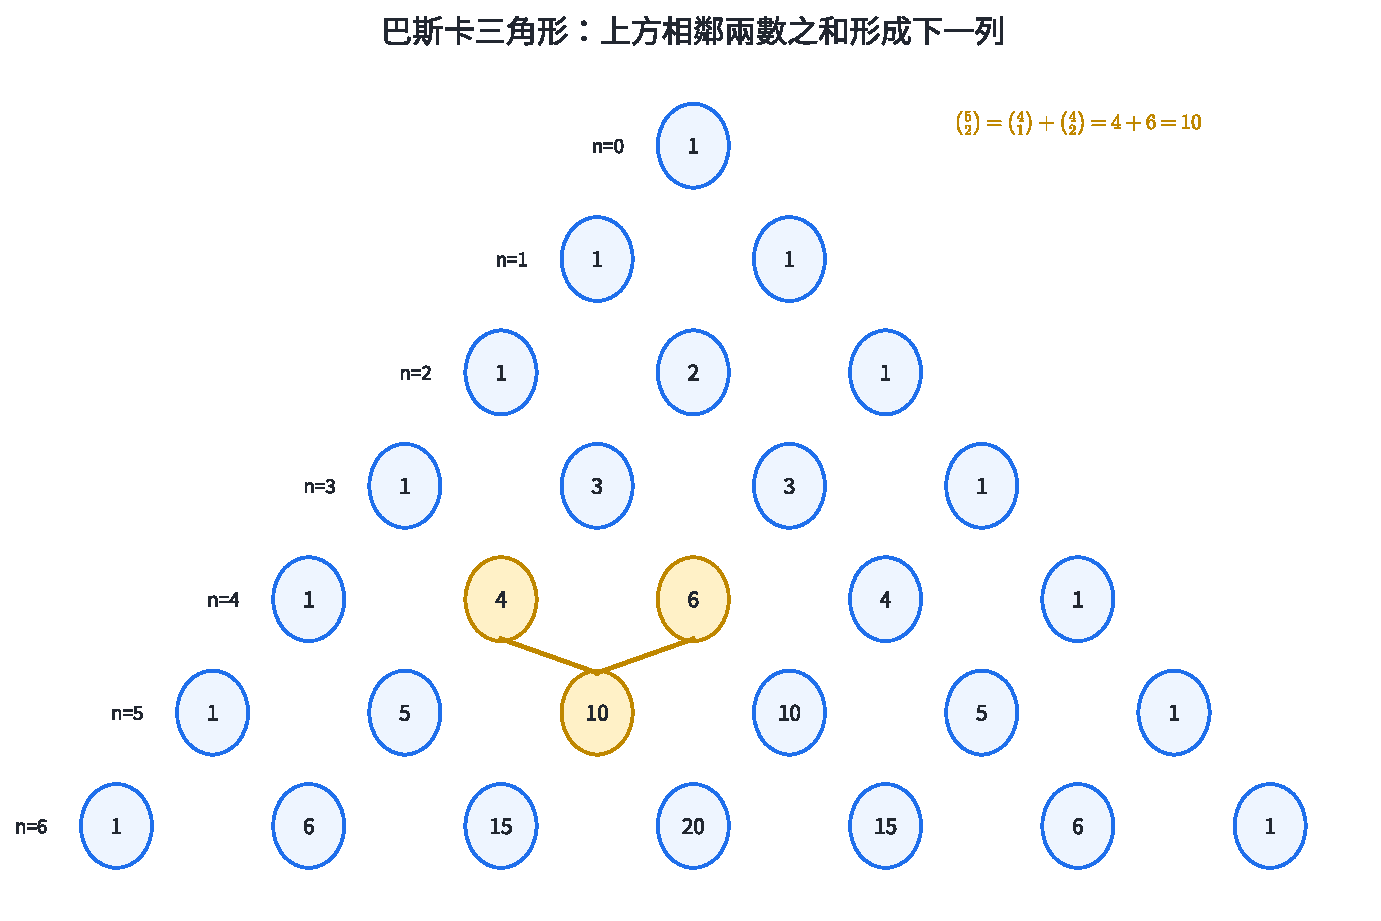
\includegraphics[width=0.82\linewidth,height=\textheight,keepaspectratio,alt={巴斯卡三角形中的每個內部數都由上方相鄰兩數相加}]{assets/數2-3-巴斯卡三角形.pdf}
\caption{巴斯卡三角形中的每個內部數都由上方相鄰兩數相加}
\end{figure}

令二項式定理中的 \(x=y=1\)，可得一列組合數之和：

\[
\sum_{k=0}^{n}\binom nk=(1+1)^n=2^n.
\]

這也等於 \(n\) 元集合的所有子集合數，因為每個元素都有「選」與「留」兩種狀態。

令 \(x=1,y=-1\)，當 \(n\ge1\) 時，

\[
\sum_{k=0}^{n}(-1)^k\binom nk=(1-1)^n=0.
\]

因此偶數索引的組合數總和等於奇數索引的組合數總和，各為 \(2^{n-1}\)。

\subsection{例 16｜用巴斯卡恆等式拆解組合數}\label{ux4f8b-16ux7528ux5df4ux65afux5361ux6046ux7b49ux5f0fux62c6ux89e3ux7d44ux5408ux6578}

計算 \(\binom83\)，並以「指定某人是否入選」解釋。

從 8 人選 3 人，指定甲。包含甲時，再選 2 人，有 \(\binom72=21\) 種；不包含甲時，從其餘 7 人選 3 人，有 \(\binom73=35\) 種。因此

\[
\binom83=\binom72+\binom73=21+35=56.
\]

\subsection{例 17｜計算一列中的奇偶索引總和}\label{ux4f8b-17ux8a08ux7b97ux4e00ux5217ux4e2dux7684ux5947ux5076ux7d22ux5f15ux7e3dux548c}

求

\[
\binom90+\binom92+\binom94+\binom96+\binom98.
\]

這是第 9 列偶數索引的總和。偶、奇索引總和相等，而整列總和是 \(2^9\)，所以答案為

\[
2^8=256.
\]

\subsection{7.2 分節練習}\label{ux5206ux7bc0ux7df4ux7fd2-6}

\begin{enumerate}
\def\labelenumi{\arabic{enumi}.}
\tightlist
\item
  用巴斯卡恆等式把 \(\binom{10}{4}\) 寫成兩個第 9 列組合數之和。
\item
  求 \(\displaystyle\sum_{k=0}^{8}\binom8k\)。
\item
  求 \(\binom{10}{1}+\binom{10}{3}+\binom{10}{5}+\binom{10}{7}+\binom{10}{9}\)。
\item
  說明 \(\binom{11}{5}=\binom{10}{4}+\binom{10}{5}\) 的分類意義。
\end{enumerate}

\subsection{7.3 分節練習解析}\label{ux5206ux7bc0ux7df4ux7fd2ux89e3ux6790-6}

\begin{enumerate}
\def\labelenumi{\arabic{enumi}.}
\tightlist
\item
  \(\binom{10}{4}=\binom93+\binom94\)。
\item
  整列總和為 \(2^8=256\)。
\item
  這是第 10 列奇數索引總和，等於 \(2^9=512\)。
\item
  從 11 人選 5 人，指定甲。包含甲時由其餘 10 人選 4 人，有 \(\binom{10}{4}\) 種；留下甲時由其餘 10 人選 5 人，有 \(\binom{10}{5}\) 種。兩類合起來就是 \(\binom{11}{5}\)。
\end{enumerate}

巴斯卡三角形把局部遞迴與全列係數連在一起，可用於快速產生二項式係數、組合恆等式與計數程式的動態更新。

\section{8. 樣本空間}\label{ux6a23ux672cux7a7aux9593}

\subsection{8.1 試驗、樣本點與樣本空間}\label{ux8a66ux9a57ux6a23ux672cux9edeux8207ux6a23ux672cux7a7aux9593}

在相同條件下可重複進行，而單次結果在進行前具有不確定性的過程稱為\textbf{隨機試驗}。一次試驗所有可能結果所成的集合稱為\textbf{樣本空間}，記作 \(S\)；其中每一個結果稱為\textbf{樣本點}。

建立樣本空間時，要先決定一個樣本點記錄哪些資訊。例如連續擲兩次硬幣，\((H,T)\) 表示第一次正面、第二次反面。時間次序屬於結果的一部分，因此

\[
S=\{(H,H),(H,T),(T,H),(T,T)\}.
\]

若從甲、乙、丙三人中選兩人組隊，交換選取先後不改變隊伍，樣本點可寫成

\[
S=\{\{\text{甲,乙}\},\{\text{甲,丙}\},\{\text{乙,丙}\}\}.
\]

同一問題的分子與分母必須使用相同結果單位。若分母把抽取順序列入樣本點，事件的有利結果也要保留順序；若分母使用無序小組，分子也使用無序小組。

\begin{figure}
\centering
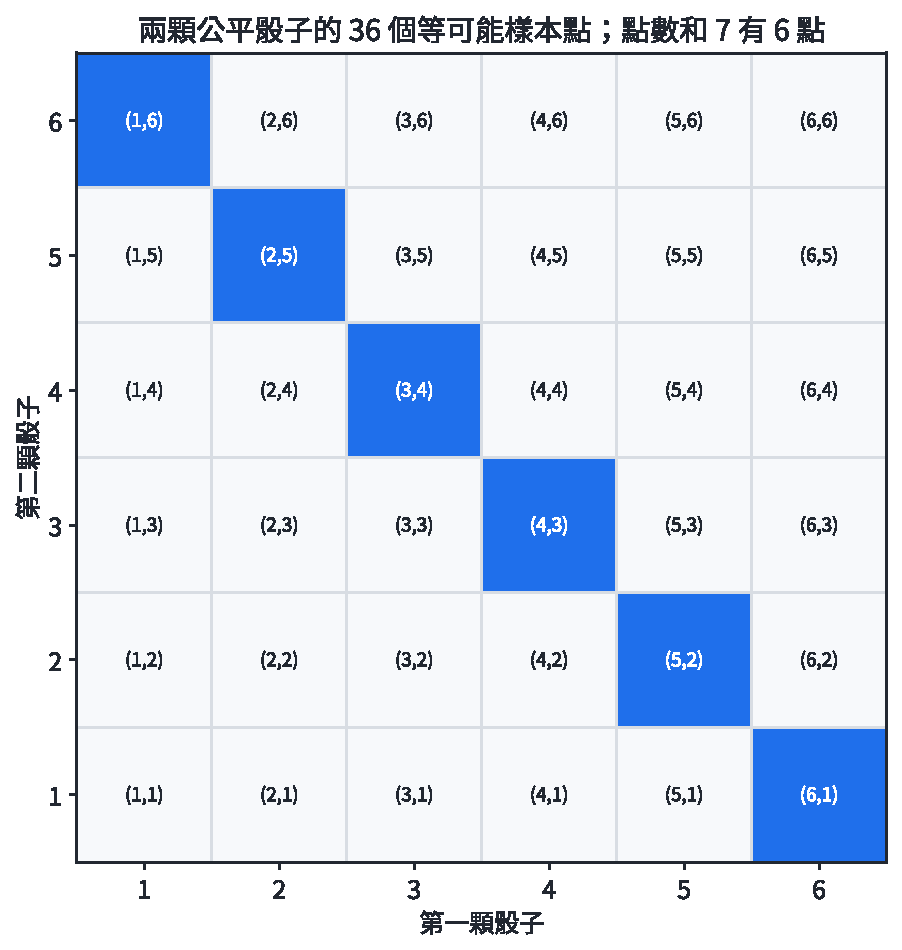
\includegraphics[width=0.78\linewidth,height=\textheight,keepaspectratio,alt={有序對把兩顆骰子的結果放入六乘六的樣本空間}]{assets/數2-3-骰子樣本空間.pdf}
\caption{有序對把兩顆骰子的結果放入六乘六的樣本空間}
\end{figure}

\subsection{例 18｜列出兩次硬幣試驗的樣本空間}\label{ux4f8b-18ux5217ux51faux5169ux6b21ux786cux5e63ux8a66ux9a57ux7684ux6a23ux672cux7a7aux9593}

擲一枚硬幣兩次，以 H、T 分別表示正面、反面。第一、二次結果形成有序對，因此

\[
S=\{HH,HT,TH,TT\},\qquad |S|=4.
\]

「恰有一次正面」對應 \(HT,TH\) 兩個樣本點。兩者都要保留，因為正面出現的時間位置不同。

\subsection{例 19｜有放回與不放回的樣本點}\label{ux4f8b-19ux6709ux653eux56deux8207ux4e0dux653eux56deux7684ux6a23ux672cux9ede}

袋中有標號 \(1,2,3\) 的球，依序抽兩次並記錄標號。

有放回時，每次都可抽到三種標號：

\[
S_{\text{有放回}}=\{(i,j):i,j\in\{1,2,3\}\},\qquad |S|=3^2=9.
\]

不放回時，第二次要排除第一次的標號：

\[
S_{\text{不放回}}=\{(i,j):i,j\in\{1,2,3\},\ i\ne j\},\qquad |S|=3\cdot2=6.
\]

\subsection{8.2 分節練習}\label{ux5206ux7bc0ux7df4ux7fd2-7}

\begin{enumerate}
\def\labelenumi{\arabic{enumi}.}
\tightlist
\item
  擲一枚硬幣三次，用 H、T 表示結果。寫出樣本空間並求大小。
\item
  同時擲一顆紅骰與一顆藍骰，以有序對記錄點數。樣本空間有幾個樣本點？
\item
  從 A、B、C、D 四人中選兩人組隊。以無序小組為樣本點，列出樣本空間。
\item
  從標號 \(1,2,3,4\) 的卡片中依序抽兩張。分別求有放回與不放回時的樣本空間大小。
\end{enumerate}

\subsection{8.3 分節練習解析}\label{ux5206ux7bc0ux7df4ux7fd2ux89e3ux6790-7}

\begin{enumerate}
\def\labelenumi{\arabic{enumi}.}
\tightlist
\item
  \(S=\{HHH,HHT,HTH,HTT,THH,THT,TTH,TTT\}\)，共有 \(2^3=8\) 點。
\item
  紅骰點數是第一座標，藍骰點數是第二座標，各有 6 種，故 \(|S|=6\cdot6=36\)。
\item
  \(S=\{\{A,B\},\{A,C\},\{A,D\},\{B,C\},\{B,D\},\{C,D\}\}\)，共有 \(\binom42=6\) 點。
\item
  有放回時兩個位置各有 4 種，大小為 \(4^2=16\)；不放回時依序有 \(4,3\) 種，大小為 \(4\cdot3=12\)。
\end{enumerate}

樣本空間是抽樣模擬、可靠度測試與機率程式的資料結構。先固定一次結果的欄位、順序與放回規則，後續事件和機率才能使用同一套結果編碼。

\section{9. 事件}\label{ux4e8bux4ef6}

\subsection{9.1 事件是樣本空間的子集合}\label{ux4e8bux4ef6ux662fux6a23ux672cux7a7aux9593ux7684ux5b50ux96c6ux5408}

樣本空間 \(S\) 的任一子集合稱為\textbf{事件}。只含一個樣本點的是單一事件；含多個樣本點的是複合事件。\(S\) 本身是必然事件，\(\emptyset\) 是不可能事件。

事件運算沿用集合語言：

\[
A\cup B:\ A\text{ 或 }B\text{ 至少一個發生},
\]

\[
A\cap B:\ A\text{ 與 }B\text{ 同時發生},
\]

\[
A^c:\ A\text{ 沒有發生}.
\]

若 \(A\cap B=\emptyset\)，稱 \(A,B\) \textbf{互斥}，表示一次試驗中兩事件無法同時發生。互斥描述交集為空；是否互斥要由樣本點檢查。

\begin{figure}
\centering
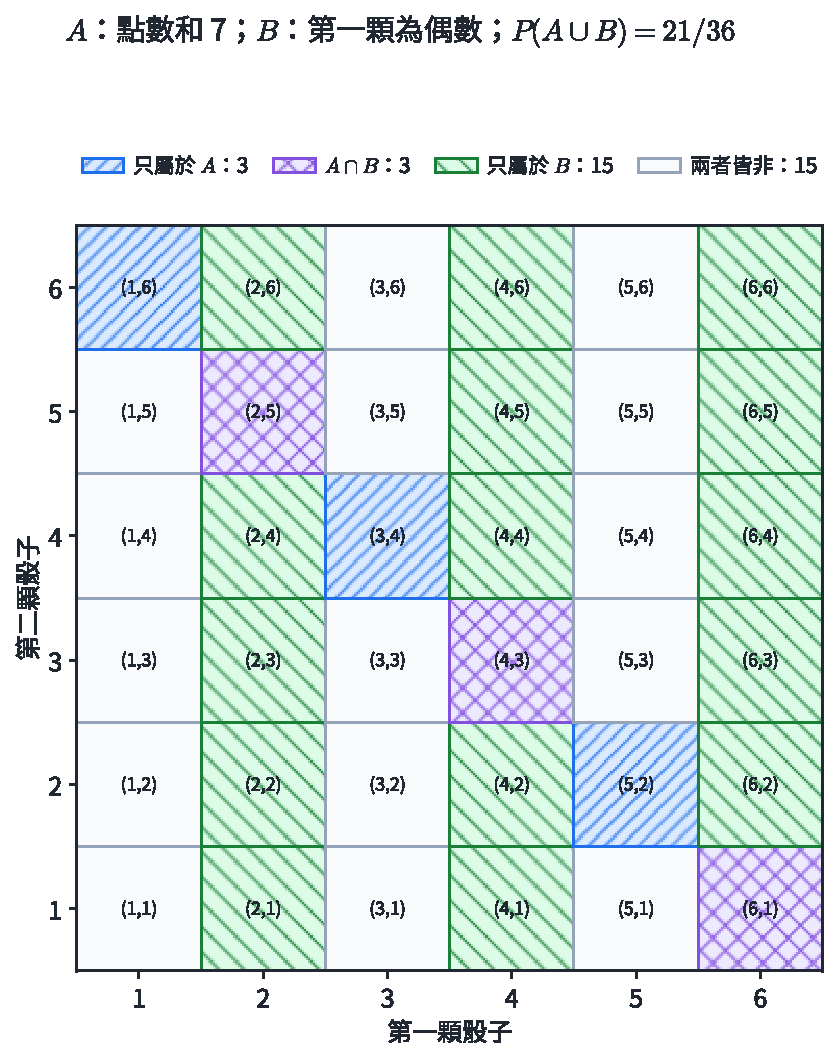
\includegraphics[width=0.88\linewidth,height=\textheight,keepaspectratio,alt={兩個骰子事件的交集、各自區域與事件外區域都由樣本點計數}]{assets/數2-3-事件區域.pdf}
\caption{兩個骰子事件的交集、各自區域與事件外區域都由樣本點計數}
\end{figure}

\subsection{例 20｜把敘述翻成事件運算}\label{ux4f8b-20ux628aux6558ux8ff0ux7ffbux6210ux4e8bux4ef6ux904bux7b97}

擲兩顆骰子。令 \(A\) 表示「點數和為 7」，\(B\) 表示「第一顆為偶數」。

\begin{itemize}
\tightlist
\item
  \(A\cap B\)：點數和為 7，且第一顆為偶數，樣本點是 \((2,5),(4,3),(6,1)\)。
\item
  \(A\cup B\)：點數和為 7，或第一顆為偶數，包含兩事件所有樣本點。
\item
  \(A^c\)：點數和不等於 7。
\end{itemize}

\(A\cap B\) 含 3 個樣本點，所以 \(A,B\) 可同時發生，兩事件不互斥。

\subsection{例 21｜互斥事件與補事件}\label{ux4f8b-21ux4e92ux65a5ux4e8bux4ef6ux8207ux88dcux4e8bux4ef6}

從一副標準撲克牌抽一張。令 \(C\) 表示抽到紅心，\(D\) 表示抽到黑桃，\(E\) 表示抽到紅色牌。

紅心與黑桃的花色不同，所以 \(C\cap D=\emptyset\)，\(C,D\) 互斥。

再令 \(F\) 表示抽到方塊。紅色牌是紅心或方塊，因此 \(E=C\cup F\)；\(E^c\) 是黑色牌，也就是黑桃或梅花。由事件笛摩根律，

\[
E^c=C^c\cap F^c.
\]

\subsection{9.2 分節練習}\label{ux5206ux7bc0ux7df4ux7fd2-8}

\begin{enumerate}
\def\labelenumi{\arabic{enumi}.}
\tightlist
\item
  擲一顆骰子，\(S=\{1,2,3,4,5,6\}\)。令 \(A\) 表示偶數，\(B\) 表示大於 4。寫出 \(A,B,A\cap B,A\cup B,A^c\)。
\item
  從 \(1\) 到 \(10\) 任取一個整數。令 \(C\) 表示 2 的倍數，\(D\) 表示 5 的倍數。判斷 \(C,D\) 是否互斥。
\item
  擲一枚硬幣兩次。令 \(E\) 表示至少一次正面，寫出 \(E\) 與 \(E^c\)。
\item
  對任意兩事件 \(A,B\)，用文字說明 \((A\cap B)^c=A^c\cup B^c\)。
\end{enumerate}

\subsection{9.3 分節練習解析}\label{ux5206ux7bc0ux7df4ux7fd2ux89e3ux6790-8}

\begin{enumerate}
\def\labelenumi{\arabic{enumi}.}
\tightlist
\item
  \(A=\{2,4,6\}\)，\(B=\{5,6\}\)，\(A\cap B=\{6\}\)，\(A\cup B=\{2,4,5,6\}\)，\(A^c=\{1,3,5\}\)。
\item
  \(C=\{2,4,6,8,10\}\)，\(D=\{5,10\}\)，交集是 \(\{10\}\)，所以兩事件不互斥。
\item
  \(S=\{HH,HT,TH,TT\}\)。\(E=\{HH,HT,TH\}\)，\(E^c=\{TT\}\)。
\item
  「\(A\) 與 \(B\) 同時發生」沒有成立，等價於「\(A\) 沒有發生或 \(B\) 沒有發生」，所以兩邊代表相同樣本點集合。
\end{enumerate}

事件把文字條件轉成樣本點集合，可直接支援品質篩選、警報規則與資料分類。交、聯、補運算也會成為下一節機率公式的結構。

\section{10. 古典機率}\label{ux53e4ux5178ux6a5fux7387}

\subsection{10.1 有限且等可能的模型}\label{ux6709ux9650ux4e14ux7b49ux53efux80fdux7684ux6a21ux578b}

若樣本空間 \(S\) 有限，而且每個樣本點發生的機會相同，事件 \(A\) 的\textbf{古典機率}定義為

\[
\boxed{P(A)=\frac{|A|}{|S|}}.
\]

這個公式的條件是樣本點等可能。公平骰子的六個點數等可能；若轉盤各區面積不同，把每個顏色區塊直接當成一個樣本點就未必等可能，需要依面積或實驗頻率另建模型。

由集合分割可推得基本性質：

\[
P(S)=1,\qquad P(\emptyset)=0,
\]

\[
\boxed{P(A^c)=1-P(A)},
\]

\[
\boxed{P(A\cup B)=P(A)+P(B)-P(A\cap B)}.
\]

第三式來自 \(A\) 與 \(A^c\) 把 \(S\) 分成兩個互斥區域；第四式則修正交集被重複計算一次。若 \(A,B\) 互斥，交集機率為 \(0\)，聯集機率可直接相加。

\subsection{10.2 用排列組合計算樣本點}\label{ux7528ux6392ux5217ux7d44ux5408ux8a08ux7b97ux6a23ux672cux9ede}

抽取、排隊與分組的機率常先用排列或組合計算 \(|S|\) 與 \(|A|\)。分子、分母必須採用一致的結果單位：兩者都記順序，或兩者都只記成員。使用組合時，通常表示每個同大小小組等可能。

\subsection{例 22｜兩顆骰子的點數和}\label{ux4f8b-22ux5169ux9846ux9ab0ux5b50ux7684ux9edeux6578ux548c}

擲兩顆公平骰子，求點數和為 7 的機率。

以有序對 \((i,j)\) 為樣本點，共有 \(6\cdot6=36\) 個等可能結果。點數和為 7 的有

\[
(1,6),(2,5),(3,4),(4,3),(5,2),(6,1),
\]

共 6 個，所以

\[
P(\text{和為 }7)=\frac6{36}=\frac16.
\]

\subsection{例 23｜不放回抽球恰好一紅一白}\label{ux4f8b-23ux4e0dux653eux56deux62bdux7403ux6070ux597dux4e00ux7d05ux4e00ux767d}

袋中有 4 顆紅球、3 顆白球，任取 2 顆，求恰好一紅一白的機率。

以無序兩球小組為樣本點，總數為 \(\binom72=21\)。有利結果先選 1 紅再選 1 白：

\[
\binom41\binom31=12.
\]

所以

\[
P(\text{一紅一白})=\frac{12}{21}=\frac47.
\]

\subsection{例 24｜至少一個事件用補集}\label{ux4f8b-24ux81f3ux5c11ux4e00ux500bux4e8bux4ef6ux7528ux88dcux96c6}

袋中有 3 顆紅球、7 顆藍球，任取 4 顆，求至少有 1 顆紅球的機率。

總樣本數為 \(\binom{10}{4}\)。「至少 1 紅」的補事件是「4 顆全藍」，所以

\[
P(\text{至少 1 紅})
=1-\frac{\binom74}{\binom{10}{4}}
=1-\frac{35}{210}
=\frac56.
\]

\subsection{例 25｜重複月份的機率}\label{ux4f8b-25ux91cdux8907ux6708ux4efdux7684ux6a5fux7387}

假設每人的出生月份在 12 個月中等可能且彼此獨立。4 人中至少兩人同月出生的機率為何？

補事件是 4 人月份都不同。全部月份序列有 \(12^4\) 種；月份都不同有 \(P^{12}_4\) 種。因此

\[
P(\text{至少同月})
=1-\frac{P^{12}_4}{12^4}
=1-\frac{12\cdot11\cdot10\cdot9}{12^4}
=\frac{41}{96}.
\]

此模型把月份視為等可能；若處理真實人口資料，可改用各月實際比例。

\subsection{10.3 分節練習}\label{ux5206ux7bc0ux7df4ux7fd2-9}

\begin{enumerate}
\def\labelenumi{\arabic{enumi}.}
\tightlist
\item
  擲一顆公平骰子，求點數為質數的機率。
\item
  擲兩顆公平骰子，求點數和至少為 10 的機率。
\item
  一副標準 52 張撲克牌中任抽一張，求抽到紅色牌或 K 的機率。
\item
  5 顆紅球、4 顆白球中任取 3 顆，求恰有 2 顆紅球的機率。
\item
  6 人中隨機選 2 人，求甲、乙至少一人入選的機率。
\item
  擲一枚公平硬幣 5 次，求至少出現一次正面的機率。
\end{enumerate}

\subsection{10.4 分節練習解析}\label{ux5206ux7bc0ux7df4ux7fd2ux89e3ux6790-9}

\begin{enumerate}
\def\labelenumi{\arabic{enumi}.}
\tightlist
\item
  質數點數是 \(2,3,5\)，共 3 個，故機率 \(3/6=1/2\)。
\item
  和為 \(10\) 有 3 點、和為 \(11\) 有 2 點、和為 \(12\) 有 1 點，共 6 點，因此機率 \(6/36=1/6\)。
\item
  紅色牌 26 張，K 有 4 張，其中紅色 K 有 2 張。由取捨公式，有利牌數 \(26+4-2=28\)，機率 \(28/52=7/13\)。
\item
  總數 \(\binom93=84\)；有利數 \(\binom52\binom41=10\cdot4=40\)，機率 \(40/84=10/21\)。
\item
  補事件是甲乙都未入選。有利於補事件的小組數為 \(\binom42=6\)，總數 \(\binom62=15\)，所以所求機率 \(1-6/15=3/5\)。
\item
  補事件是五次全反面，機率為 \((1/2)^5=1/32\)，所以至少一次正面的機率是 \(31/32\)。
\end{enumerate}

古典機率用於抽樣檢驗、隨機分派、遊戲與簡化風險模型。計算前先確認樣本點是否等可能，再用計數原理建立同一尺度的分子與分母。

\section{11. 期望值}\label{ux671fux671bux503c}

\subsection{11.1 機率分布與長期平均}\label{ux6a5fux7387ux5206ux5e03ux8207ux9577ux671fux5e73ux5747}

把隨機試驗的每個結果對應到一個數值，就得到隨機變數 \(X\)。若 \(X\) 的可能值為 \(x_1,x_2,\ldots,x_k\)，對應機率為 \(p_1,p_2,\ldots,p_k\)，其中

\[
p_i\ge0,\qquad p_1+p_2+\cdots+p_k=1,
\]

則 \(X\) 的\textbf{期望值}是

\[
\boxed{E(X)=x_1p_1+x_2p_2+\cdots+x_kp_k}.
\]

若同一試驗重複很多次，約有比例 \(p_i\) 的試驗得到 \(x_i\)。總值除以試驗次數後，便接近 \(\sum x_ip_i\)，因此期望值描述長期每次試驗的平均值。

\begin{figure}
\centering
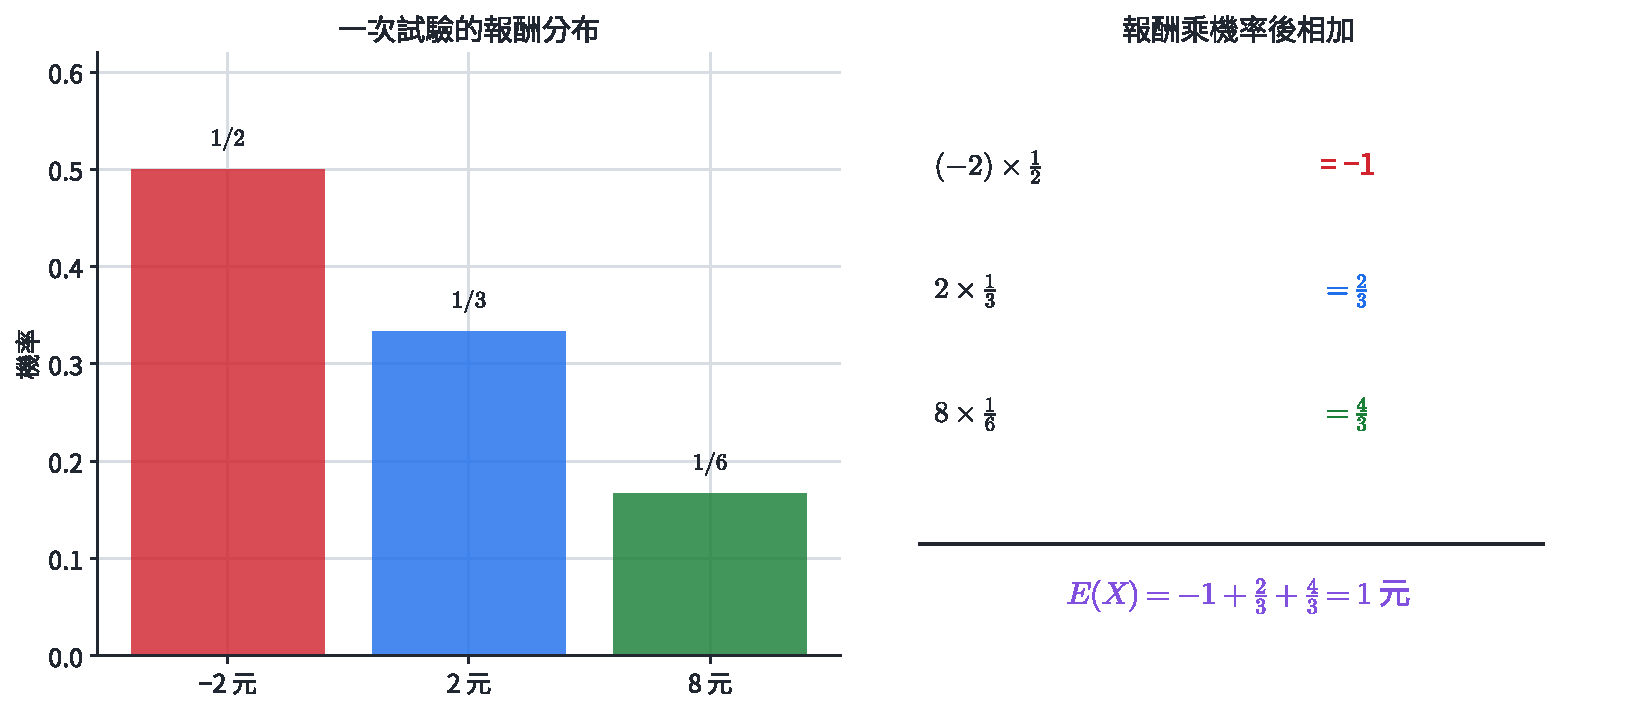
\includegraphics[width=0.92\linewidth,height=\textheight,keepaspectratio,alt={每種報酬乘上發生機率後相加，得到每次試驗的長期平均}]{assets/數2-3-期望值分布.pdf}
\caption{每種報酬乘上發生機率後相加，得到每次試驗的長期平均}
\end{figure}

期望值可以不等於任何一次實際結果。例如公平骰子的點數期望值是 \(3.5\)，雖然單次不會擲出 \(3.5\) 點；\(3.5\) 表示大量重複後的平均點數。

若遊戲以淨收益為隨機變數，\(E(X)=0\) 稱為\textbf{公平遊戲}；正值表示參與者長期平均獲利，負值表示長期平均損失。

\subsection{例 26｜由報酬分布計算期望值}\label{ux4f8b-26ux7531ux5831ux916cux5206ux5e03ux8a08ux7b97ux671fux671bux503c}

擲一顆公平骰子。點數 \(1,2,3\) 得 \(-2\) 元，點數 \(4,5\) 得 \(2\) 元，點數 \(6\) 得 \(8\) 元。求期望淨收益。

三類互斥且涵蓋全部，機率依序為 \(3/6,2/6,1/6\)，所以

\[
E(X)=(-2)\frac36+2\frac26+8\frac16
=-1+\frac23+\frac43=1.
\]

長期平均每次淨收益為 1 元。

\subsection{例 27｜由公平條件反求扣分}\label{ux4f8b-27ux7531ux516cux5e73ux689dux4ef6ux53cdux6c42ux6263ux5206}

一道單選題有 5 個選項。答對得 4 分，答錯扣 \(x\) 分，完全隨機作答時希望期望得分為 0。求 \(x\)。

答對機率為 \(1/5\)，答錯機率為 \(4/5\)，所以

\[
4\cdot\frac15+(-x)\cdot\frac45=0.
\]

乘以 5 得 \(4-4x=0\)，故

\[
x=1.
\]

\subsection{例 28｜抽票券的平均回饋}\label{ux4f8b-28ux62bdux7968ux5238ux7684ux5e73ux5747ux56deux994b}

盒中有 10 張等可能票券：1 張回饋 100 元、3 張回饋 20 元、6 張回饋 0 元。每抽一次的期望回饋是多少？若每次需付 18 元，期望淨收益是多少？

期望回饋為

\[
100\cdot\frac1{10}+20\cdot\frac3{10}+0\cdot\frac6{10}=16\text{ 元}.
\]

扣除固定費用 18 元，期望淨收益為

\[
16-18=-2\text{ 元}.
\]

\subsection{11.2 分節練習}\label{ux5206ux7bc0ux7df4ux7fd2-10}

\begin{enumerate}
\def\labelenumi{\arabic{enumi}.}
\tightlist
\item
  公平骰子的點數 \(X\) 可能為 \(1\) 到 \(6\)，求 \(E(X)\)。
\item
  一枚公平硬幣擲一次，正面得 6 元、反面損失 2 元，求期望淨收益。
\item
  某產品抽樣後有 \(0.7\) 機率成本為 10 元、\(0.2\) 機率成本為 30 元、\(0.1\) 機率成本為 80 元，求期望成本。
\item
  袋中 5 張票券等可能，獎金依序為 \(0,0,10,20,50\) 元。每抽一次收費多少元時，期望淨收益為 0？
\item
  一場遊戲有 \(1/4\) 機率得 12 分，其餘情況扣 \(a\) 分。若期望得分為 0，求 \(a\)。
\end{enumerate}

\subsection{11.3 分節練習解析}\label{ux5206ux7bc0ux7df4ux7fd2ux89e3ux6790-10}

\begin{enumerate}
\def\labelenumi{\arabic{enumi}.}
\tightlist
\item
  \(E(X)=(1+2+3+4+5+6)/6=21/6=3.5\)。
\item
  \(E(X)=6(1/2)+(-2)(1/2)=2\) 元。
\item
  \(E(X)=10(0.7)+30(0.2)+80(0.1)=7+6+8=21\) 元。
\item
  期望獎金為 \((0+0+10+20+50)/5=16\) 元。收費 16 元時，期望淨收益為 \(16-16=0\)。
\item
  \(12(1/4)+(-a)(3/4)=0\)，乘以 4 得 \(12-3a=0\)，所以 \(a=4\) 分。
\end{enumerate}

期望值用於比較長期平均成本、收益與計分規則。它只保留平均位置；若兩個方案的波動幅度不同，完整比較還需同時查看各結果機率與可能損失範圍。

\section{12. 章末分層題}\label{ux7ae0ux672bux5206ux5c64ux984c}

\subsection{12.1 基礎與核心題}\label{ux57faux790eux8207ux6838ux5fc3ux984c}

\begin{enumerate}
\def\labelenumi{\arabic{enumi}.}
\item
  討論範圍為實數。令 \(P:x>3\)，\(Q:x^2>9\)。判斷 \(P\Rightarrow Q\) 與 \(Q\Rightarrow P\)，並寫出「\(x>3\) 且 \(x\le10\)」的否定。
\item
  令 \(U=\{1,2,\ldots,15\}\)，\(A\) 是 3 的倍數集合，\(B\) 是質數集合。求 \(A\cap B\)、\(A\cup B\) 與 \((A\cup B)^c\)。
\item
  \(1\) 到 \(300\) 中，能被 \(4\) 或 \(9\) 整除的整數有幾個？
\item
  從 \(0,1,2,\ldots,7\) 中取 5 個不同數字排成五位數，共有幾個？
\item
  STATISTICS 的 10 個字母共有幾種不同排列？
\item
  用 6 種顏色塗 5 個排成一列的色塊，相鄰色塊顏色不同，共有幾種？
\item
  6 位男生與 5 位女生中選 5 人，至少有 2 位女生，共有幾種？
\item
  求 \(\left(x^2-\dfrac2x\right)^6\) 的常數項。
\item
  求

  \[
  \binom{11}{1}+\binom{11}{3}+\binom{11}{5}+\binom{11}{7}+\binom{11}{9}+\binom{11}{11}.
  \]
\item
  擲一枚公平硬幣三次。寫出「恰有兩次正面」事件及其補事件，並求兩事件各含多少個樣本點。
\item
  5 顆紅球與 4 顆白球中任取 3 顆，求至少取到 1 顆白球的機率。
\item
  隨機變數 \(X\) 以機率 \(1/2,1/3,1/6\) 分別取值 \(-4,2,a\)。若 \(E(X)=0\)，求 \(a\)。
\end{enumerate}

\subsection{12.2 跨節整合題}\label{ux8de8ux7bc0ux6574ux5408ux984c}

\begin{enumerate}
\def\labelenumi{\arabic{enumi}.}
\setcounter{enumi}{12}
\tightlist
\item
  甲、乙等 6 人隨機排成一列。求甲乙不相鄰的排列數與機率。
\item
  從 \(1\) 到 \(180\) 隨機選一個整數。令 \(A\) 表示選到 6 的倍數，\(B\) 表示選到 10 的倍數。求 \(P(A\cup B)\)、恰有一事件發生的機率，以及兩事件都不發生的機率。
\item
  把 BANANA 的不同字母排列等可能地選出一個。求三個 A 兩兩不相鄰的排列數與機率。
\item
  袋中有 3 顆紅球、2 顆藍球，不放回任取 2 顆。兩紅得 12 分，一紅一藍得 4 分，兩藍扣 \(x\) 分。列出分數的機率分布，並求遊戲公平時的 \(x\)。
\end{enumerate}

\section{13. 章末題完整詳解}\label{ux7ae0ux672bux984cux5b8cux6574ux8a73ux89e3}

\subsection{第 1 題}\label{ux7b2c-1-ux984c}

若 \(x>3\)，平方後必有 \(x^2>9\)，所以 \(P\Rightarrow Q\) 成立。取 \(x=-4\)，則 \(x^2=16>9\)，但 \(x>3\) 不成立，因此 \(Q\Rightarrow P\) 不成立。\(P\) 是 \(Q\) 的充分條件，\(Q\) 是 \(P\) 的必要條件。

令 \(R:x>3\)、\(T:x\le10\)。原命題是 \(R\wedge T\)，否定是

\[
(\neg R)\vee(\neg T),
\]

即

\[
x\le3\quad\text{或}\quad x>10.
\]

\subsection{第 2 題}\label{ux7b2c-2-ux984c}

\[
A=\{3,6,9,12,15\},
\]

\[
B=\{2,3,5,7,11,13\}.
\]

所以

\[
A\cap B=\{3\},
\]

\[
A\cup B=\{2,3,5,6,7,9,11,12,13,15\}.
\]

由全集移除聯集中的元素，得到

\[
(A\cup B)^c=\{1,4,8,10,14\}.
\]

元素個數檢查：\(|A\cup B|=5+6-1=10\)，其補集有 \(15-10=5\) 個，與列出的結果一致。

\subsection{第 3 題}\label{ux7b2c-3-ux984c}

4 的倍數有

\[
\left\lfloor\frac{300}{4}\right\rfloor=75
\]

個；9 的倍數有 \(\lfloor300/9\rfloor=33\) 個。兩類交集是 \(\operatorname{lcm}(4,9)=36\) 的倍數，共 \(\lfloor300/36\rfloor=8\) 個。由取捨原理，答案為

\[
75+33-8=100.
\]

\subsection{第 4 題}\label{ux7b2c-4-ux984c}

最高位決定五位數能否成立。最高位可從 \(1\) 到 \(7\) 選，有 7 種；選完後，第二位可用剩餘 7 個數字，包括 0。其後三位依序有 \(6,5,4\) 種。因此

\[
7\cdot7\cdot6\cdot5\cdot4=5880.
\]

\subsection{第 5 題}\label{ux7b2c-5-ux984c}

STATISTICS 共 10 個字母，其中 S 有 3 個、T 有 3 個、I 有 2 個，A、C 各 1 個。不同排列數為

\[
\frac{10!}{3!3!2!}
=\frac{3628800}{72}
=50400.
\]

\subsection{第 6 題}\label{ux7b2c-6-ux984c}

第一格有 6 種顏色。第二格到第五格各要與前一格不同，因此各有 5 種。總數是

\[
6\cdot5^4=3750.
\]

此條件只比較相鄰兩格，所以較早使用過的顏色可再次出現。

\subsection{第 7 題}\label{ux7b2c-7-ux984c}

依女生人數分成 2、3、4、5 人四個互斥類別：

\[
\begin{aligned}
N
&=\binom52\binom63+\binom53\binom62
 +\binom54\binom61+\binom55\binom60\\
&=10\cdot20+10\cdot15+5\cdot6+1\\
&=381.
\end{aligned}
\]

\subsection{第 8 題}\label{ux7b2c-8-ux984c}

二項式通項為

\[
\binom6k(x^2)^{6-k}\left(-\frac2x\right)^k
=\binom6k(-2)^k x^{12-3k}.
\]

常數項要求 \(12-3k=0\)，所以 \(k=4\)。代入得

\[
\binom64(-2)^4=15\cdot16=240.
\]

\subsection{第 9 題}\label{ux7b2c-9-ux984c}

題式是第 11 列所有奇數索引組合數之和。由

\[
(1+1)^{11}=\sum_{k=0}^{11}\binom{11}{k}=2^{11}
\]

與

\[
(1-1)^{11}=\sum_{k=0}^{11}(-1)^k\binom{11}{k}=0,
\]

偶數索引總和與奇數索引總和相等，各為

\[
2^{10}=1024.
\]

\subsection{第 10 題}\label{ux7b2c-10-ux984c}

三次硬幣試驗的樣本空間有 \(2^3=8\) 點。「恰有兩次正面」事件為

\[
A=\{HHT,HTH,THH\},
\]

所以 \(|A|=3\)。補事件包含正面次數為 \(0,1,3\) 的結果：

\[
A^c=\{TTT,HTT,THT,TTH,HHH\},
\]

故 \(|A^c|=5\)。兩者個數相加為 8，涵蓋整個樣本空間。

\subsection{第 11 題}\label{ux7b2c-11-ux984c}

以無序 3 球小組為樣本點，總數是 \(\binom93=84\)。至少 1 顆白球的補事件是三顆全紅，有 \(\binom53=10\) 種。因此

\[
P(\text{至少 1 白})
=1-\frac{\binom53}{\binom93}
=1-\frac{10}{84}
=\frac{37}{42}.
\]

\subsection{第 12 題}\label{ux7b2c-12-ux984c}

三個機率相加為 \(1/2+1/3+1/6=1\)。由期望值條件，

\[
(-4)\frac12+2\frac13+a\frac16=0.
\]

乘以 6：

\[
-12+4+a=0,
\]

所以

\[
\boxed{a=8}.
\]

\subsection{第 13 題｜排列與機率}\label{ux7b2c-13-ux984cux6392ux5217ux8207ux6a5fux7387}

全部排列有 \(6!=720\) 種。甲乙相鄰時，把甲乙視為一塊：外部 5 個單位有 \(5!\) 種，塊內有 \(2!\) 種，因此相鄰排列有

\[
5!2!=240
\]

種。不相鄰排列數為

\[
720-240=480.
\]

所有 6 人排列等可能，所以

\[
P(\text{甲乙不相鄰})=\frac{480}{720}=\frac23.
\]

\subsection{第 14 題｜集合、取捨與機率}\label{ux7b2c-14-ux984cux96c6ux5408ux53d6ux6368ux8207ux6a5fux7387}

樣本空間是 \(1\) 到 \(180\)，共有 180 個等可能整數。

\[
|A|=\left\lfloor\frac{180}{6}\right\rfloor=30,
\qquad
|B|=\left\lfloor\frac{180}{10}\right\rfloor=18.
\]

交集是 \(\operatorname{lcm}(6,10)=30\) 的倍數，所以 \(|A\cap B|=6\)。因此

\[
P(A\cup B)=\frac{30+18-6}{180}
=\frac{42}{180}=\frac7{30}.
\]

恰有一事件發生的個數為

\[
(30-6)+(18-6)=36,
\]

所以機率是 \(36/180=1/5\)。兩事件都不發生是 \((A\cup B)^c\)，其機率為

\[
1-\frac7{30}=\frac{23}{30}.
\]

\subsection{第 15 題｜相同物排列、空隙與機率}\label{ux7b2c-15-ux984cux76f8ux540cux7269ux6392ux5217ux7a7aux9699ux8207ux6a5fux7387}

BANANA 的全部不同排列有

\[
\frac{6!}{3!2!}=60
\]

種。為使三個 A 兩兩不相鄰，先排列 B、N、N。因兩個 N 相同，排法有

\[
\frac{3!}{2!}=3
\]

種。每種排列形成 4 個空隙：

\[
\_\ B\ \_\ N\ \_\ N\ \_.
\]

從 4 個空隙選 3 個，各放一個相同的 A，有 \(\binom43=4\) 種。因此有利排列數為

\[
3\cdot4=12.
\]

等可能選取一個不同排列時，所求機率為

\[
\frac{12}{60}=\frac15.
\]

\subsection{第 16 題｜組合機率與公平期望}\label{ux7b2c-16-ux984cux7d44ux5408ux6a5fux7387ux8207ux516cux5e73ux671fux671b}

以無序兩球小組為樣本點，總數為

\[
\binom52=10.
\]

各類結果為

\[
P(\text{兩紅})=\frac{\binom32}{\binom52}=\frac3{10},
\]

\[
P(\text{一紅一藍})=\frac{\binom31\binom21}{\binom52}=\frac6{10},
\]

\[
P(\text{兩藍})=\frac{\binom22}{\binom52}=\frac1{10}.
\]

機率總和為 \(3/10+6/10+1/10=1\)。分數分布是 \(12,4,-x\)，對應以上三個機率。公平條件為

\[
12\cdot\frac3{10}+4\cdot\frac6{10}+(-x)\cdot\frac1{10}=0.
\]

乘以 10 得

\[
36+24-x=0,
\]

所以

\[
\boxed{x=60}.
\]

\section{14. 核心整理}\label{ux6838ux5fc3ux6574ux7406}

{\def\LTcaptype{none} % do not increment counter
\begin{longtable}[]{@{}
  >{\raggedright\arraybackslash}p{(\linewidth - 4\tabcolsep) * \real{0.3333}}
  >{\raggedright\arraybackslash}p{(\linewidth - 4\tabcolsep) * \real{0.3333}}
  >{\raggedright\arraybackslash}p{(\linewidth - 4\tabcolsep) * \real{0.3333}}@{}}
\toprule\noalign{}
\begin{minipage}[b]{\linewidth}\raggedright
結構
\end{minipage} & \begin{minipage}[b]{\linewidth}\raggedright
判定方式
\end{minipage} & \begin{minipage}[b]{\linewidth}\raggedright
核心式
\end{minipage} \\
\midrule\noalign{}
\endhead
\bottomrule\noalign{}
\endlastfoot
邏輯與集合 & 且、或、否定對應交、聯、補 & \(\neg(P\wedge Q)\Leftrightarrow\neg P\vee\neg Q\)；\((A\cap B)^c=A^c\cup B^c\) \\
互斥分類 & 從不同類別擇一 & 加法原理 \\
連續步驟 & 每個結果要完成所有步驟 & 乘法原理 \\
聯集計數 & 類別有交集 & \(|A\cup B|=|A|+|B|-|A\cap B|\) \\
排列 & 次序、職務或位置有差別 & \(P^n_r=n!/(n-r)!\) \\
相同物排列 & 同類物件交換後結果相同 & \(n!/(m_1!\cdots m_k!)\) \\
重複排列 & 有序位置可重複取用 & \(n^r\) \\
組合 & 只記錄選到哪些對象 & \(\binom nr=n!/[r!(n-r)!]\) \\
二項式係數 & 從 \(n\) 個因子選 \(k\) 個提供第二項 & \((x+y)^n=\sum\binom nkx^{n-k}y^k\) \\
巴斯卡恆等式 & 依指定元素選入或留下分類 & \(\binom nk=\binom{n-1}{k-1}+\binom{n-1}{k}\) \\
古典機率 & 有限且等可能的樣本點 & \(P(A)=|A|/|S|\) \\
補事件與聯集 & 用事件區域拆分 & \(P(A^c)=1-P(A)\)；\(P(A\cup B)=P(A)+P(B)-P(A\cap B)\) \\
期望值 & 數值乘機率後加總 & \(E(X)=\sum x_ip_i\) \\
\end{longtable}
}

排列組合先回答「共有多少種」，機率再回答「有利結果在等可能結果中占多少」，期望值最後把每種數值結果依機率加權。三者共用同一項要求：先清楚定義一次結果的身分、順序與限制條件。


\end{document}
